% ============================================================================
% LDRD FFA@CEBAF Permanent Magnet Radiation Damage Study
% Comprehensive Technical Note
% ============================================================================
\documentclass[11pt,letterpaper]{article}

% --- Packages ---
\usepackage[margin=1in]{geometry}
\usepackage{graphicx}
\usepackage{amsmath,amssymb}
\usepackage{booktabs}
\usepackage{siunitx}
\usepackage{hyperref}
\usepackage{xcolor}
\usepackage{caption}
\usepackage{subcaption}
\usepackage{float}
\usepackage{multirow}
\usepackage{longtable}
\usepackage{enumitem}
\usepackage{fancyhdr}
\usepackage{appendix}
\usepackage[backend=biber,style=numeric-comp,sorting=none]{biblatex}
\addbibresource{references.bib}

% --- Page style ---
\pagestyle{fancy}
\fancyhf{}
\lhead{LDRD FFA@CEBAF Magnet Radiation Study}
\rhead{Technical Note -- DRAFT}
\cfoot{\thepage}

% --- Custom commands ---
\newcommand{\NdFeB}{Nd\textsubscript{2}Fe\textsubscript{14}B}
\newcommand{\SmCo}{Sm\textsubscript{2}Co\textsubscript{17}}
\newcommand{\ndfeb}{NdFeB}
\newcommand{\smco}{SmCo}
\newcommand{\Tc}{T_\mathrm{c}}
\newcommand{\Ha}{H_\mathrm{a}}
\newcommand{\Hci}{H_\mathrm{ci}}
\newcommand{\Br}{B_\mathrm{r}}
\newcommand{\alphar}{\alpha(\Br)}
\newcommand{\CEBAF}{CEBAF}
\newcommand{\FFA}{FFA}
\newcommand{\JLab}{Jefferson Lab}
\newcommand{\SEM}{SEM}
\newcommand{\sigstat}{\sigma_\mathrm{stat}}
\newcommand{\sigsyst}{\sigma_\mathrm{syst}}
\newcommand{\sigcomb}{\sigma_\mathrm{comb}}

\sisetup{separate-uncertainty=true}

% ============================================================================
\begin{document}

% --- Title ---
\begin{titlepage}
\centering
\vspace*{2cm}
{\Huge\bfseries Radiation-Induced Demagnetization of\\[6pt]
Permanent Magnets in the CEBAF Tunnel:\\[6pt]
A Comprehensive Technical Note}\\[1.5cm]
{\Large LDRD FFA@CEBAF Magnet Radiation Resiliency Study}\\[2cm]
{\large R.\ Bodenstein and Collaborators}\\[0.5cm]
{\large Thomas Jefferson National Accelerator Facility}\\[0.5cm]
{\large Newport News, Virginia 23606}\\[2cm]
{\large\today}\\[1cm]
{\large\textcolor{red}{DRAFT -- Internal Technical Note -- Not for Public Distribution}}\\[2cm]

\begin{abstract}
\noindent
This technical note presents the complete methodology, analysis, and results of
the LDRD (Laboratory Directed Research \& Development) study investigating
radiation-induced demagnetization of permanent magnets deployed in the Continuous
Electron Beam Accelerator Facility (\CEBAF) tunnel at \JLab. The study was
designed to determine whether Fixed Field Alternating-gradient (\FFA) accelerator
magnets, which rely on permanent magnet technology, can survive the radiation
environment at \CEBAF. Thirty Y-plates, each carrying four randomized permanent
magnet grades (two \NdFeB{}: N42EH and N52SH; two \SmCo{}: SmCo33H and SmCo35),
were deployed at seven tunnel locations for approximately 18~months, with nine
additional Y-plates kept in the lab as unexposed controls. The primary
measurement is a gain-immune intra-plate differential between the
radiation-sensitive (\ndfeb{}) and radiation-hard (\smco{}) materials, which
cancels the dominant Helmholtz coil gain drift systematic by construction. We
report a differential of $-0.208\% \pm 0.028\%$~(stat) $\pm\,0.033\%$~(syst),
corresponding to $7.6\sigma$ statistical and $4.6\sigma$ combined significance.
Lab controls confirm a null result ($-0.007\% \pm 0.038\%$, $0.2\sigma$), and
the tunnel-minus-lab excess is independently significant at $4.3\sigma$. Neutron
dose correlates with degradation ($\rho = 0.389$, $p = 0.03$) while gamma dose
does not ($\rho = 0.21$, $p = 0.27$), providing the first in-situ accelerator
confirmation of the established neutron-dominated damage hierarchy. This is the
world's largest study of radiation-induced permanent magnet demagnetization, with
a sample size ($N = 39$ plates, $156+$ individual magnets) that exceeds prior
published work by an order of magnitude.
\end{abstract}
\end{titlepage}

\tableofcontents
\newpage

% ============================================================================
\section{Introduction}
\label{sec:intro}
% ============================================================================

\subsection{Motivation}

The Continuous Electron Beam Accelerator Facility (\CEBAF) at Thomas Jefferson
National Accelerator Facility (\JLab) is a multi-pass recirculating electron
linac that delivers continuous-wave electron beams at energies up to
\SI{12}{GeV} for nuclear and particle physics experiments. A proposed upgrade
path for \CEBAF involves the use of Fixed Field Alternating-gradient (\FFA)
optics in the recirculating arcs. \FFA designs rely on permanent magnets to
generate the alternating-gradient field profiles that enable multi-energy beam
transport without the power consumption and operational complexity of
conventional electromagnets.

However, permanent magnets are known to be susceptible to radiation-induced
demagnetization. The \CEBAF tunnel is a mixed radiation environment, with both
gamma and neutron radiation fields generated by beam losses at various locations
(aperture restrictions, collimators, septa, and beam dumps). If the radiation
levels at \FFA magnet locations are sufficient to cause measurable
demagnetization over the operational lifetime of the accelerator, this would be
a fundamental obstacle to the \FFA upgrade. Similar radiation concerns have
been raised for the CBETA energy recovery linac at Cornell, where Kostroun and
Gulliford~\cite{Kostroun2019} used MCNP simulations to estimate radiation
limits on permanent magnets.

Preliminary results from this study have been reported at
IPAC2024~\cite{Bodenstein2024a,Bodenstein2024b} and
IPAC2025~\cite{Bodenstein2025}. The central question is simple: \textit{Do
permanent magnets lose measurable magnetic strength after 18~months of
parasitic exposure in the \CEBAF tunnel?}

\subsection{Why This Study Is Needed}

The existing literature on radiation damage to permanent magnets is extensive
(see Section~\ref{sec:literature} for a detailed review), but it has a critical
gap in the dose regime relevant to \CEBAF operations:

\begin{itemize}
    \item \textbf{High-dose studies} \cite{Simos2018,Bizen2016,Alderman}
    typically irradiate magnets at doses of
    \SIrange{e4}{e7}{Gy}, far above the \SIrange{0.3}{23451}{Gy} accumulated
    in the \CEBAF tunnel over 18~months.
    \item \textbf{Null results} at moderate doses are often reported as simply
    ``no effect observed,'' without quantifying the detection sensitivity.
    \item \textbf{No prior study} has used a co-located differential design
    with radiation-sensitive and radiation-hard materials on the same plate,
    measured in the same instrument session, to achieve sub-percent sensitivity
    in a real accelerator environment.
\end{itemize}

This study fills this gap by deploying a large number of carefully designed
multi-material sample plates directly in the \CEBAF tunnel, measuring them with
a gain-immune technique, and comparing to matched laboratory controls.

\subsection{Scope of This Document}

This technical note is a comprehensive record of the entire study. It covers:

\begin{enumerate}
    \item The experimental design and sample configuration (Section~\ref{sec:design})
    \item The measurement methodology and instrumentation (Section~\ref{sec:measurement})
    \item The temperature correction procedure and its evolution (Section~\ref{sec:temperature})
    \item The dosimetry pipeline (Section~\ref{sec:dosimetry})
    \item The primary results (Section~\ref{sec:results})
    \item Dose-degradation correlations (Section~\ref{sec:dose_degradation})
    \item The complete systematic error analysis and uncertainty budget (Section~\ref{sec:systematics})
    \item Comparison to theoretical models (Section~\ref{sec:theory})
    \item Context within the published literature (Section~\ref{sec:literature})
    \item Remaining work and future directions (Section~\ref{sec:future})
\end{enumerate}

The intended audience ranges from subject matter experts in accelerator physics
and radiation effects to graduate students and advanced undergraduates beginning
work in this field. Accordingly, we explain both the ``what'' and the ``why'' of
every analysis decision.

% ============================================================================
\section{Experimental Design}
\label{sec:design}
% ============================================================================

\subsection{Overview}

The study uses three types of sample assemblies, each designed for a different
measurement approach:

\begin{description}[style=nextline]
    \item[Y-plates (primary measurement)]
    Large single magnets measured with a Helmholtz coil fluxmeter. Each Y-plate
    has four material slots, one each of the four magnet grades (N42EH, N52SH,
    SmCo33H, SmCo35), with \textbf{randomized slot assignments}. This
    randomization is critical: it ensures that any position-dependent
    measurement artifact averages out across the ensemble. Thirty Y-plates were
    deployed in the \CEBAF tunnel; nine were kept in the laboratory as
    unexposed controls.

    \item[H-plates (pair assemblies)]
    Each H-plate contains four pair slots in one of four magnetic
    configurations: Alpha ($0^\circ$, aligned), Beta ($180^\circ$,
    antiparallel), Gamma ($90^\circ$, perpendicular), and Delta
    (single pair with calibration slug). These configurations were specifically
    chosen to approximate the range of field orientations present in a Halbach
    array: Alpha represents aligned flux regions, Beta (antiparallel) simulates
    adjacent reverse-flux wedges, and Gamma (perpendicular) probes the
    intermediate orientation where non-uniform degradation patterns differ from
    both parallel and antiparallel cases~\cite{NGotta2024,Brooks2017}.
    NdFeB pairs are on ``n'' plates (Hn-XX-Y), SmCo on ``s'' plates
    (Hs-XX-Y). Unlike Y-plates, NdFeB and SmCo H-plates are \emph{not}
    co-located on the same physical plate, which means H-plate measurements
    are \emph{not} gain-immune.

    \item[A-samples (individual magnets)]
    Pairs of small magnets measured together in a fixed enclosure, extracted
    from H-plate assemblies. Named An-XX-Y-Z (NdFeB) or As-XX-Y-Z (SmCo).
    These provide the finest-granularity measurement but with the highest
    noise.
\end{description}

\subsection{Material Selection}
\label{sec:materials}

Four permanent magnet grades were selected, spanning two material families:

\begin{table}[H]
\centering
\caption{Material specifications from Allstar Magnetics datasheets. All magnets
were custom-manufactured for this study.}
\label{tab:materials}
\begin{tabular}{@{}lcccccc@{}}
\toprule
\textbf{Grade} & \textbf{Family} & $\Br$ (kGs) & $\Hci$ (kOe) &
$T_\mathrm{max}$ (\si{\celsius}) & $\alphar$ (\%/\si{\celsius}) &
$\Tc$ (\si{\celsius}) \\
\midrule
N42EH  & \NdFeB  & 12.8--13.2 & $\geq 30$ & 190 & $-0.10$ & $\sim 315$ \\
N52SH  & \NdFeB  & 14.2--14.5 & $\geq 19$ & 140 & $-0.11$ & $\sim 315$ \\
SmCo33H & \SmCo  & 11.2--11.5 & $\geq 25$ & 350 & $-0.040$ & $\sim 820$ \\
SmCo35  & \SmCo  & 11.6--12.0 & $\geq 18$ & 300 & $-0.040$ & $\sim 820$ \\
\bottomrule
\end{tabular}
\end{table}

\textbf{Why these four grades?} The two material families (\ndfeb{} and \smco{})
have fundamentally different radiation resistance due to their Curie
temperatures: \NdFeB{} has $\Tc \approx \SI{588}{K}$ while \SmCo{} has $\Tc
\approx \SI{1093}{K}$. This nearly factor-of-two difference means that the
thermal spike volume exceeding $\Tc$ after a neutron interaction is much
smaller in \smco{}, making it substantially more radiation-resistant. Within
each family, two grades with different coercivities ($\Hci$) were chosen:
\begin{itemize}
    \item N42EH has high $\Hci \geq \SI{30}{kOe}$ (achieved by
    dysprosium addition; Allstar composition data: 1--2\,wt\%\,Dy, 3--5\,wt\%\,Tb)
    \item N52SH has moderate $\Hci \geq \SI{19}{kOe}$ (\textbf{zero} Dy,
    2--4\,wt\%\,Tb, with high $\Br$ prioritized)
    \item SmCo33H has $\Hci \geq \SI{25}{kOe}$
    \item SmCo35 has $\Hci \geq \SI{18}{kOe}$
\end{itemize}

The expectation from the thermal spike model (Section~\ref{sec:theory}) was
that higher $\Hci$ would correlate with greater radiation resistance. As we
will discuss, this prediction holds for the \smco{} grades but is
\textbf{inverted} for the \ndfeb{} grades, a finding with important
mechanistic implications.

\subsection{Slot Randomization}

Each Y-plate has four slots. The four material grades were assigned to these
slots using a randomization procedure \emph{before deployment}. This means
that, across the ensemble of 30 tunnel plates:
\begin{itemize}
    \item Each material appears at each slot position approximately equally
    often
    \item Any systematic bias associated with slot position (e.g., edge effects
    in the Helmholtz coil) averages out in the ensemble mean
    \item The analyst had no control over which material occupied which position,
    eliminating selection bias
\end{itemize}

\subsection{Tunnel Deployment}
\label{sec:deployment}

The 30 tunnel Y-plates were deployed at seven locations within the \CEBAF
accelerator, chosen to span a wide range of radiation environments:

\begin{table}[H]
\centering
\caption{Summary of tunnel deployment locations. Each Y-plate is co-located
with one H-plate for cross-checking. Arc plates are arranged in stacks of five,
with each line position corresponding to a different beam energy pass.}
\label{tab:deployment}
\begin{tabular}{@{}lccc@{}}
\toprule
\textbf{Region} & \textbf{N (Y-plates)} & \textbf{Arrangement} & \textbf{Dose Range (Gy)} \\
\midrule
SE Arc    & 5 & Stack of 5, upstream Girder 27 & $\sim$30--1200 \\
NE Arc    & 5 & Stack of 5, above JD3A06 area & $\sim$30--1200 \\
NW Arc    & 5 & Stack of 5, above MJC4A24 area & $\sim$30--1200 \\
SW Arc    & 5 & Stack of 5, above MJC4A14 area & $\sim$30--1200 \\
North Linac & 4 & At NDX girder locations & $\sim$300--23,451 \\
South Linac & 4 & At NDX girder locations & $\sim$80--3000 \\
Labyrinths  & 2 & Access tunnel controls & $\sim$0.3--10 \\
\bottomrule
\end{tabular}
\end{table}

\textbf{Arc stacks.} In each of the four recirculating arcs (SE, NE, NW, SW),
five Y-plates are stacked vertically. Each physical line position (Line~1
through Line~5, top to bottom) corresponds to a different beam energy pass.
Line~1 (top) carries the lowest-energy beam, which has the lowest magnetic
rigidity and therefore the largest beam envelope; as we will see, this is the location showing the
most degradation. This spatial structure is important for understanding the
dose-position inversion discussed in Section~\ref{sec:position_inversion}.

\textbf{Linac locations.} Plates in the North and South Linacs are positioned
near neutron detector (NDX) locations at specific girders. These locations
experience the highest gamma doses in the study (\SI{\sim 23}{kGy} at Y-22 in
the North Linac), driven by high beam current and proximity to beam loss
points.

\textbf{Labyrinths.} Two plates (Y-12 at North, Y-20 at South) are in the
access labyrinths, which are shielded locations with very low dose rates. These serve as
low-dose controls within the tunnel environment.

\subsection{Lab Controls}

Nine Y-plates (plates 8, 14, 27, 28, 29, 31, 33, 35, 37) were stored in
laboratory boxes throughout the study period with zero radiation exposure. They
underwent the \textbf{identical measurement protocol} (same Helmholtz coil,
same Teslameter, same measurement schedule) as the tunnel plates. Any
systematic effect of the measurement procedure itself (e.g., aging, thermal
cycling, magnetic relaxation) would appear equally in both tunnel and lab
plates. The lab controls therefore provide a clean null hypothesis: if the
measurement system is unbiased, lab plates should show zero
material-dependent differential.

\subsection{Study Timeline}

\begin{itemize}
    \item \textbf{April--November 2024}: Pre-deployment baseline measurements
    (lab). Multiple sessions per plate to establish reliable baselines.
    \item \textbf{July 2025}: Magnets deployed in the \CEBAF tunnel.
    \item \textbf{July 2025--January 2026}: Post-deployment measurement
    campaigns (periodic removal for measurement, then return to tunnel).
    \item \textbf{Total exposure}: $\sim$18 months of parasitic radiation
    during normal beam operations.
\end{itemize}

% ============================================================================
\section{Measurement Methodology}
\label{sec:measurement}
% ============================================================================

\subsection{Helmholtz Coil Fluxmeter}

The primary measurement instrument is a Helmholtz coil coupled to a Fluxmeter
Model~2130. A Helmholtz coil consists of two identical circular coils separated
by a distance equal to their radius, producing a highly uniform magnetic field
region at the center. When a permanent magnet sample is inserted into (or
removed from) this region, the change in magnetic flux through the coils
induces an electromotive force (EMF) that is integrated by the fluxmeter to
yield a reading proportional to the sample's magnetic moment.

\textbf{Key properties:}
\begin{itemize}
    \item \textbf{Integrating measurement}: The Helmholtz coil integrates over
    the entire sample volume. Unlike a point-measurement magnetometer, the
    result is largely independent of the exact position of the sample within
    the coil, as long as it is approximately centered.
    \item \textbf{Gain drift}: The fluxmeter exhibits session-to-session gain
    drift of $\sim$0.5--0.7\%, meaning the absolute reading can shift by this
    amount between measurement sessions. This is the single largest
    instrumental systematic for absolute measurements. However, as we will
    discuss, this drift \textbf{cancels} in the intra-plate differential.
    \item \textbf{DC accuracy}: The Fluxmeter Model~2130 has a specified DC
    accuracy of 0.050\% (typical) to 0.100\% (maximum) of full scale. This
    sets an absolute accuracy floor but is common-mode for all samples
    measured in the same session.
    \item \textbf{Readings in mWC}: The raw output is in units of
    milliWeber-centimeter (mWC), proportional to the magnetic moment.
\end{itemize}

\subsection{Teslameter Temperature Measurement}

A SENIS 3MH6-E Teslameter with an integrated Hall probe provides temperature
readings at the measurement location. These temperatures are used for the
temperature correction described in Section~\ref{sec:temperature}.

\textbf{Important: single instrument.} There is only one Teslameter with one
Hall probe at any given time. Y-plates, H-plates, and A-samples all use the
\textbf{same device}. The original probe broke and was replaced between
December~2024 and July~2025 (before tunnel deployment). Therefore, any
temperature differences between Y and H measurements on the same day reflect
measurement timing and room conditions, not different instruments.

The Teslameter is used \emph{only} for temperature readings in this analysis,
not for the demagnetization measurement. The Teslameter's positioning noise
(0.14--1.9\% depending on face orientation) is irrelevant to the Helmholtz
results.

\subsection{Measurement Protocol}

Each measurement session follows a standardized protocol:
\begin{enumerate}
    \item Power on the Helmholtz coil and fluxmeter; allow thermal equilibration.
    \item Record ambient temperature via Teslameter.
    \item For each Y-plate:
    \begin{enumerate}
        \item Insert sample into Helmholtz coil.
        \item Record integrated flux reading (mWC).
        \item Record Teslameter temperature.
        \item Repeat for all four material slots.
    \end{enumerate}
    \item Record any instrument anomalies or environmental changes.
\end{enumerate}

\textbf{Critical point}: All four magnet slots on a given Y-plate are measured
in the \textbf{same session}, minutes apart, sharing the same gain state of the
Helmholtz coil. This is what makes the intra-plate differential gain-immune.

\subsection{The Gain-Immune Intra-Plate Differential}
\label{sec:gain_immune}

This is the most important methodological concept in the study. It deserves
careful explanation.

Consider a single Y-plate with four magnets. In a given measurement session,
the Helmholtz coil has some gain factor $G$ (ideally 1.000, but drifting by
$\sim$0.5\% session-to-session). The measured flux for each magnet is:
\begin{equation}
    M_i = G \cdot H_i(T)
\end{equation}
where $H_i(T)$ is the true magnetic moment of magnet $i$ at temperature $T$.
The percentage change from baseline for each magnet is:
\begin{equation}
    \Delta_i = \frac{M_i^\mathrm{post} - M_i^\mathrm{pre}}{M_i^\mathrm{pre}} \times 100\%
    = \frac{G^\mathrm{post} H_i^\mathrm{post} - G^\mathrm{pre} H_i^\mathrm{pre}}{G^\mathrm{pre} H_i^\mathrm{pre}} \times 100\%
\end{equation}

If we now compute the \emph{differential} between the NdFeB mean and SmCo mean
\emph{on the same plate}:
\begin{equation}
    \delta = \overline{\Delta}_\mathrm{NdFeB} - \overline{\Delta}_\mathrm{SmCo}
    = \frac{1}{2}(\Delta_\mathrm{N42EH} + \Delta_\mathrm{N52SH})
    - \frac{1}{2}(\Delta_\mathrm{SmCo33H} + \Delta_\mathrm{SmCo35})
\end{equation}

Because all four magnets share the same gain factors $G^\mathrm{pre}$ and
$G^\mathrm{post}$ in their respective sessions, any multiplicative gain change
cancels in the difference \emph{to first order}. This is analogous to
common-mode rejection in electronics: the ``signal'' is the material-dependent
radiation effect, and the ``noise'' is the gain drift, which is common to all
channels.

\textbf{Quantitative impact}: Without this cancellation, each material
measurement carries a $\pm 0.124\%$ gain systematic. With the intra-plate
differential, the gain systematic is \textbf{zero by construction}, and the
measurement is limited by the $\pm 0.028\%$ statistical uncertainty, a factor
of $\sim$4.4 improvement in precision.

The \textbf{headline result} of this study is always this gain-immune
intra-plate differential, computed from the 30 tunnel Y-plates.

\subsection{Percentage Change Calculation}

For each magnet slot, the percentage change from baseline is:
\begin{equation}
    \Delta_i = \frac{H_\mathrm{latest}(T_\mathrm{ref}) - \overline{H}_\mathrm{baseline}(T_\mathrm{ref})}{\overline{H}_\mathrm{baseline}(T_\mathrm{ref})} \times 100\%
    \label{eq:pct_change}
\end{equation}
where $H(T_\mathrm{ref})$ denotes the Helmholtz reading after correction to the
reference temperature $T_\mathrm{ref} = \SI{20}{\celsius}$ (see
Section~\ref{sec:temperature}), and $\overline{H}_\mathrm{baseline}$ is the
mean of all pre-deployment baseline readings for that slot.

A \textbf{negative} $\Delta_i$ indicates demagnetization (loss of magnetic
moment). The sentinel value 1337 in raw data files indicates a missing or
invalid measurement and is excluded before any calculations.

% ============================================================================
\section{Temperature Correction}
\label{sec:temperature}
% ============================================================================

\subsection{Why Temperature Matters}

Permanent magnets have a temperature-dependent remanence. As temperature
increases, the magnetic moment decreases reversibly (for small excursions around
ambient). This relationship is parameterized by the temperature coefficient of
remanence, $\alphar$:
\begin{equation}
    \Br(T) = \Br(T_0) \left[ 1 + \alphar (T - T_0) \right]
\end{equation}

For our materials, $\alphar$ ranges from $-0.040$\%/\si{\celsius} (\smco{})
to $-0.11$\%/\si{\celsius} (N52SH). This means a \SI{1}{\celsius} difference
between the baseline and post-deployment measurement temperatures shifts the
apparent percentage change by $-0.04$ to $-0.11$\%.

\textbf{The key problem}: The pre-deployment baseline measurements were
conducted in the laboratory at temperatures that were not directly and
precisely measured at the time. The Teslameter probe readings provide
approximate temperatures, but the probe was later found to have a systematic
bias of approximately $+\SI{0.8}{\celsius}$ relative to the true room
temperature. Getting this baseline temperature right is the single largest
systematic uncertainty in the analysis.

\subsection{Temperature Correction Formula}

All Helmholtz readings are corrected to a common reference temperature of
$T_\mathrm{ref} = \SI{20}{\celsius}$:
\begin{equation}
    H_\mathrm{corrected} = \frac{H_\mathrm{raw}}{1 + \alphar (T_\mathrm{measured} - T_\mathrm{ref})}
    \label{eq:temp_correction}
\end{equation}

The temperature coefficients used are the manufacturer-specified values from
Allstar Magnetics (Table~\ref{tab:materials}).

\subsection{Evolution of the Temperature Correction}
\label{sec:temp_history}

Three successive versions of the temperature correction were applied as our
understanding of the baseline temperatures improved. Documenting this evolution
is important for transparency and for understanding the robustness of the
result.

\subsubsection{Version~1 (v1): Raw probe temperatures}

The initial analysis used the Teslameter probe temperatures directly. For
pre-deployment dates (November~2024), probe readings were $\sim$24.6--\SI{26.7}{\celsius}. This
produced the largest differential:
\begin{equation*}
    \delta_\mathrm{v1} = -0.266\% \pm 0.028\%~(\mathrm{stat}) \quad [9.6\sigma]
\end{equation*}

\textbf{Problem}: The probe readings were later found to be biased
$\sim$\SI{0.8}{\celsius} high relative to an independent temperature reference
(see Section~\ref{sec:probe_bias}).

\subsubsection{Version~2 (v2): Blanket \SI{23}{\celsius} correction}

A second analysis applied a uniform correction, assuming all baseline
measurements were at \SI{23}{\celsius}. This was based on an initial (incorrect)
estimate that the probe was $\sim$\SI{2}{\celsius} high.
\begin{equation*}
    \delta_\mathrm{v2} = -0.134\% \pm 0.028\%~(\mathrm{stat}) \quad [4.9\sigma]
\end{equation*}

\textbf{Problem}: This overcorrected. SmCo33H showed an anomalously positive
change ($+0.083\%$, $2.7\sigma$), which is physically implausible for a
radiation-hard material.

\subsubsection{Version~3 (v3, current): Per-date calibrated estimates}

The current analysis uses data-driven, per-date temperature estimates based on
same-day Y--H measurement comparisons. This is the best-justified approach:

\begin{table}[H]
\centering
\caption{Per-date baseline temperature estimates used in the v3 analysis. For
dates with same-day H-plate measurements, the H temperature is used directly.
For Y-only dates, the measured $+\SI{0.8}{\celsius}$ probe bias is subtracted.}
\label{tab:temp_v3}
\begin{tabular}{@{}lcccc@{}}
\toprule
\textbf{Date} & \textbf{Y Probe (\si{\celsius})} &
\textbf{Correction} & \textbf{Est.\ True $T$ (\si{\celsius})} &
\textbf{Source} \\
\midrule
Nov 5, 2024  & 25.1 & $-0.8$ (probe bias) & 24.3 & Pooled same-day evidence \\
Nov 7, 2024  & 24.6 & $-0.8$ (probe bias) & 23.8 & Pooled same-day evidence \\
Nov 20, 2024 & 25.4 & Direct H reading    & 24.6 & Same-day H = \SI{24.62}{\celsius} \\
Sep 30, 2024 & 26.7 & Direct H reading    & 25.8 & Same-day H = \SI{25.80}{\celsius} \\
\bottomrule
\end{tabular}
\end{table}

\begin{equation*}
    \delta_\mathrm{v3} = -0.208\% \pm 0.028\%~(\mathrm{stat}) \quad [7.6\sigma]
\end{equation*}

\textbf{Why v3 is best}:
\begin{enumerate}
    \item \textbf{Data-driven}: Uses same-day Y--H cross-checks, not
    assumptions about room temperature.
    \item \textbf{Physically sensible}: SmCo near zero ($+0.037\%$ and
    $-0.044\%$), both \ndfeb{} clearly negative, N42EH~$>$~N52SH.
    \item \textbf{Robust}: The signal exceeds $5\sigma$ for \emph{any}
    baseline temperature in the \SIrange{23}{25}{\celsius} range.
\end{enumerate}

\subsection{Probe Bias Assessment}
\label{sec:probe_bias}

Only two pre-deployment dates have both Y-plate and H-plate readings with the
same probe:

\begin{table}[H]
\centering
\caption{Same-day Y--H temperature comparisons. The Y--H difference of
$\sim$\SI{0.8}{\celsius} is explained by measurement timing (Y measured
$\sim$1~hour later, when the room was slightly warmer).}
\label{tab:probe_bias}
\begin{tabular}{@{}lccccc@{}}
\toprule
\textbf{Date} & Y mean (\si{\celsius}) & H mean (\si{\celsius}) & Y$-$H (\si{\celsius}) & Time gap \\
\midrule
Sep 30, 2024 & 26.66 & 25.80 & $+0.87$ & Y $\sim$1.3\,h later \\
Nov 20, 2024 & 25.38 & 24.62 & $+0.77$ & Y $\sim$0.9\,h later \\
\bottomrule
\end{tabular}
\end{table}

The mean Y--H difference is $+\SI{0.82}{\celsius}$, not the $+\SI{2}{\celsius}$
initially assumed. The earlier estimate was based on comparing Y readings on
Nov~5/7 to an H reading on Dec~4, but \textbf{these are different days} with
different room temperatures. The Dec~4 H reading (\SI{22.8}{\celsius}) was
simply a cold day.

For comparison, tunnel-era data (new probe, near-simultaneous Y/H measurements)
shows Y$-$H $= -0.15\pm\SI{0.14}{\celsius}$ across 10 dates, confirming that
same-probe, same-time differences are small.

\subsection{Temperature Sensitivity}
\label{sec:temp_sensitivity}

The differential depends linearly on the assumed baseline temperature:
\begin{equation}
    \frac{\partial \delta}{\partial T_\mathrm{baseline}} = -0.066\%/\si{\celsius}
    \label{eq:temp_sensitivity}
\end{equation}

This slope follows directly from the difference in temperature coefficients:
\begin{equation}
    \Delta\alpha = \overline{\alphar}_\mathrm{NdFeB} - \overline{\alphar}_\mathrm{SmCo}
    = \left(\frac{-0.10 + (-0.11)}{2}\right) - (-0.040)
    = -0.065\%/\si{\celsius}
\end{equation}

The predicted $-0.065\%/\si{\celsius}$ matches the observed
$-0.066\%/\si{\celsius}$ from a numerical scan, confirming internal
consistency.

Table~\ref{tab:temp_scan} shows how the differential varies across the
plausible temperature range:

\begin{table}[H]
\centering
\caption{Differential and significance as a function of assumed baseline
temperature. The signal exceeds $5\sigma$ for the entire \SIrange{23}{25}{\celsius}
range.}
\label{tab:temp_scan}
\begin{tabular}{@{}ccc@{}}
\toprule
\textbf{Assumed $T$ (\si{\celsius})} & \textbf{Differential (\%)} & \textbf{Significance} \\
\midrule
23.0 (v2) & $-0.134$ & $5.0\sigma$ \\
23.5      & $-0.166$ & $6.1\sigma$ \\
24.0      & $-0.199$ & $7.2\sigma$ \\
$\sim$24.1 (v3) & $-0.208$ & $7.6\sigma$ \\
24.5      & $-0.231$ & $8.4\sigma$ \\
25.0      & $-0.264$ & $9.6\sigma$ \\
\bottomrule
\end{tabular}
\end{table}

\subsection{Temperature Coefficient Uncertainty}

The manufacturer specifies $\alphar$ values with a relative uncertainty of
$\pm$5--10\% per grade (worst case $\pm$20\%). An empirical measurement was
attempted using the temperature variation of tunnel readings across
measurement dates, but Teslameter positioning jig noise
(0.14--1.9\% standard deviation depending on face) dominated the
$\sim$0.4--0.9\% temperature signal over the $\sim$\SI{9}{\celsius} span,
producing slopes that scattered from 10\% to 184\% of nominal. A dedicated
temperature sweep without removing magnets from the jig would be needed to
improve this.

The impact on the differential is small:

\begin{table}[H]
\centering
\caption{Impact of temperature coefficient ($\alphar$) uncertainty on results.}
\label{tab:alpha_uncertainty}
\begin{tabular}{@{}lccc@{}}
\toprule
$\alphar$ tolerance & Differential shift & Individual shift & Assessment \\
\midrule
$\pm$10\% & $\pm$0.014\% & $\pm$0.021\% & Negligible vs.\ stat ($\pm$0.028\%) \\
$\pm$20\% (worst) & $\pm$0.028\% & $\pm$0.042\% & Comparable to stat, still negligible vs.\ gain \\
\bottomrule
\end{tabular}
\end{table}

% ============================================================================
\section{Dosimetry}
\label{sec:dosimetry}
% ============================================================================

Understanding the radiation environment at each sample location is essential
for interpreting the degradation results. Two independent dosimetry systems
were deployed alongside the magnet samples, supplemented by data from the
facility's area monitoring program.

\subsection{Dosimetry Systems Overview}

\begin{description}[style=nextline]
    \item[OSL Badges (Landauer InLight 2T + CR-39)]
    Optically Stimulated Luminescence (OSL) badges are the standard personnel
    and area dosimeters used at \JLab. Each badge contains an OSL element for
    photon/beta dosimetry and a CR-39 plastic track-etch detector for neutron
    dosimetry. The OSL element saturates at \SI{1000}{rad} (\SI{10}{Gy}),
    which means that for many tunnel locations (particularly linac and arc
    positions) the photon dose is only a \textbf{lower bound}. The CR-39
    neutron detector survives to higher doses and provides separate thermal
    and fast neutron readings.

    Across all 11 Landauer xlsx reports, there are 1,576 total rows covering
    1,330 unique badge part numbers. Only 78 of these could be directly mapped
    to LDRD plate locations via the SpareAreas.txt lookup file; full mapping
    requires the RADCON database (Part\# $\to$ Area Number $\to$ physical
    location), which remains incomplete.

    \item[FWT-70 Optichromic Rods (AIdata)]
    FWT-70 rods are passive gamma dosimeters based on radiation-induced color
    changes in a dyed polymer film. Each plate location has four rods (two
    low-range, two high-range) that are read spectrophotometrically at two
    wavelengths (600\,nm and 656\,nm). The rods have a much higher dynamic
    range than OSL badges (\SIrange{2}{726}{krad}, or \SIrange{20}{7260}{Gy}),
    making them essential for the high-dose linac and arc locations where OSL
    saturates.

    The rod data was compiled by Kirsten (the dosimetry lead) into an ``AIdata''
    database that applies a cascading best-of decision tree per swap period:
    \begin{enumerate}
        \item If Low@600 $< \SI{2}{krad}$ and OSL not saturated: use OSL.
        \item If Low@600 $< \SI{2}{krad}$ and OSL saturated: fill with
        \SI{1.5}{krad} (gap estimate).
        \item If \SIrange{2}{12}{krad}: average two Low@600 readings.
        \item If Low@600 $>$ \SI{12}{krad} and High@600 $>$ \SI{12}{krad}:
        average two High@600 readings.
        \item At higher doses: include Low@656 and High@600/656.
        \item At very high doses: average Low@656(2) + High@656(2).
    \end{enumerate}
    This methodology ensures that the most reliable rod reading is always
    selected for the dose range encountered.

    \item[Neutron Dosimetry (CR-39 Track Etch)]
    Neutron doses are measured by the CR-39 component of the OSL badges. After
    etching, the density and size of nuclear recoil tracks provide separate
    estimates of thermal and fast neutron dose. The thermal/fast breakdown from
    the Landauer PDF reports is stored in \texttt{neutron\_breakdown.csv} and
    was used for the fast vs.\ thermal neutron correlation analysis
    (Section~\ref{sec:fast_thermal}).
\end{description}

\subsection{Dose Ranges and Key Numbers}

The AIdata rod measurements provide the authoritative gamma doses. The range
spans five orders of magnitude:

\begin{table}[H]
\centering
\caption{Gamma dose ranges by tunnel region, from AIdata rod measurements
(FWT-70 optichromic rods). Note that OSL readings are lower bounds for most
tunnel locations due to saturation.}
\label{tab:dose_ranges}
\begin{tabular}{@{}lcc@{}}
\toprule
\textbf{Region} & \textbf{Gamma Dose Range (Gy)} & \textbf{OSL Status} \\
\midrule
North Linac    & 300--23,451 & Mostly saturated \\
South Linac    & 80--3,000   & Mostly saturated \\
Arcs (SE/NE/NW/SW) & 30--7,000 & Mixed \\
Labyrinths     & 0.3--30     & Unsaturated \\
\bottomrule
\end{tabular}
\end{table}

The highest single-plate dose is \SI{23451}{Gy} at Y-22 (North Linac,
Girder~26). For context, this is still \textbf{300$\times$ below} the
\SI{7}{MGy} gamma null result of Alderman et al.~\cite{Alderman} at ANL, and well below the
$>$\SI{100}{kGy} doses used in most deliberate irradiation studies.

\subsection{Rod Dosimetry Pipeline}

Building the dosimetry database required a six-phase pipeline, implemented in
Python scripts in the \texttt{Rod\_Dosimetry/} directory:

\begin{enumerate}
    \item \textbf{Rod mapping} (\texttt{rod\_mapping.py}): Parse 52,000+
    \texttt{.dat} measurement files to extract R-\#\#\# rod identifiers from
    the Notes field. This maps 736 unique R-\#\#\# rod IDs to 60 plates.

    \item \textbf{Rod spreadsheet parsing} (\texttt{parse\_rod\_spreadsheet.py}):
    Parse the optichromic rod OD (optical density) measurements and apply
    calibration curves to convert OD to dose. Of 1,358 LDRD rods, 495 (36.5\%)
    have valid readings within the calibrated range (\SIrange{2}{726}{krad}).

    \item \textbf{AIdata parsing} (\texttt{parse\_aidata.py}): Extract Kirsten's
    pre-integrated cumulative doses from the AIdata spreadsheet. Output: 61
    plates with cumulative photon and neutron doses.

    \item \textbf{Cross-checking} (\texttt{rod\_crosscheck.py}): Three-way
    validation between AIdata, independently parsed rod doses, and OSL badges.
    Key verification: AIdata units confirmed as REM by exact match with
    unsaturated OSL readings (Y-12: 31.251~rem $=$ 31,251~mrem, 0.000\% delta).

    \item \textbf{Merged dose table} (\texttt{build\_merged\_dose.py}):
    Authoritative per-plate dose table merging all sources using a hierarchical
    decision tree.

    \item \textbf{Dose--degradation merge} (\texttt{rod\_dose\_correlation.py}):
    Combine dose data with per-plate degradation results for correlation
    analysis.
\end{enumerate}

\subsection{Rod Calibration and Uncertainty}
\label{sec:rod_calibration}

The FWT-70 rods are read by measuring optical density (OD) at 600\,nm and
656\,nm, then converting to dose via calibration curves. The calibration was
characterized in Task~22 of this study:

\begin{itemize}
    \item \textbf{Independent calibration fits}: Four OD-to-dose calibration
    curves were fit independently (Low@600, Low@656, High@600, High@656),
    achieving $R^2 = 0.85$--$1.00$ (plot C1).

    \item \textbf{Replicate OD spread}: When two rods of the same type are
    read at the same location, the median relative difference between replicates
    is 5--11\% (from 2,716 replicate pairs). This is the dominant source of
    per-reading uncertainty.

    \item \textbf{Kirsten's reported uncertainty} ($\sim$15\% typical) vs.\
    our independent estimate ($\sim$6\% median) differ because Kirsten
    propagates additional calibration uncertainty.

    \item \textbf{Uncertainty budget}: For the 9 OSL-matched plates (where
    AIdata uses OSL directly), a 10\% Landauer fallback uncertainty is applied.
    For the 21 rod-derived plates, Kirsten's propagated sigma is used. Full
    uncertainty budgets are in \texttt{uncertainty\_budget.txt} and
    \texttt{rod\_uncertainty\_budget.csv}.
\end{itemize}

\subsection{Neutron Dose}

Neutron doses come from the CR-39 component of the Landauer badges. The total
neutron dose and the thermal/fast breakdown are available for most plates.

\begin{itemize}
    \item \textbf{Median fast/thermal ratio}: 12.5 (range 9--16), meaning fast
    neutrons dominate the spectrum at \CEBAF.
    \item \textbf{29 of 30} tunnel Y-plates have positive fast and thermal
    neutron readings. Y-17 reports zero for both.
    \item \textbf{Neutron quality factor}: The Landauer reports give dose in
    mrem (dose equivalent), with the quality factor $Q$ applied internally.
    For fast neutrons, $Q \approx 10$ (ICRP~60~\cite{ICRP60} at $\sim$\SI{1}{MeV}); for
    thermal neutrons, $Q = 2.5$ (10~CFR~20). Converting to absorbed dose (Gy)
    introduces a factor-of-2 systematic from the assumed spectrum.
\end{itemize}

% ============================================================================
\section{Primary Results}
\label{sec:results}
% ============================================================================

\subsection{Headline Result: NdFeB--SmCo Differential}

The gain-immune intra-plate differential from 30 tunnel Y-plates, corrected
to per-date baseline temperatures ($\sim$\SI{24}{\celsius}), is:

\begin{equation}
\boxed{
    \delta = -0.208\% \pm 0.028\%~(\mathrm{stat}) \pm 0.033\%~(\mathrm{syst})
    \quad [7.6\sigma~\mathrm{stat},\; 4.6\sigma~\mathrm{combined}]
}
\label{eq:headline}
\end{equation}

The negative sign indicates that \ndfeb{} lost more magnetic moment than
\smco{} during the $\sim$18-month tunnel exposure. Because \smco{} is expected
to be radiation-hard (Section~\ref{sec:theory}), this differential is
interpreted as radiation-induced demagnetization of \ndfeb{}.

\begin{figure}[H]
    \centering
    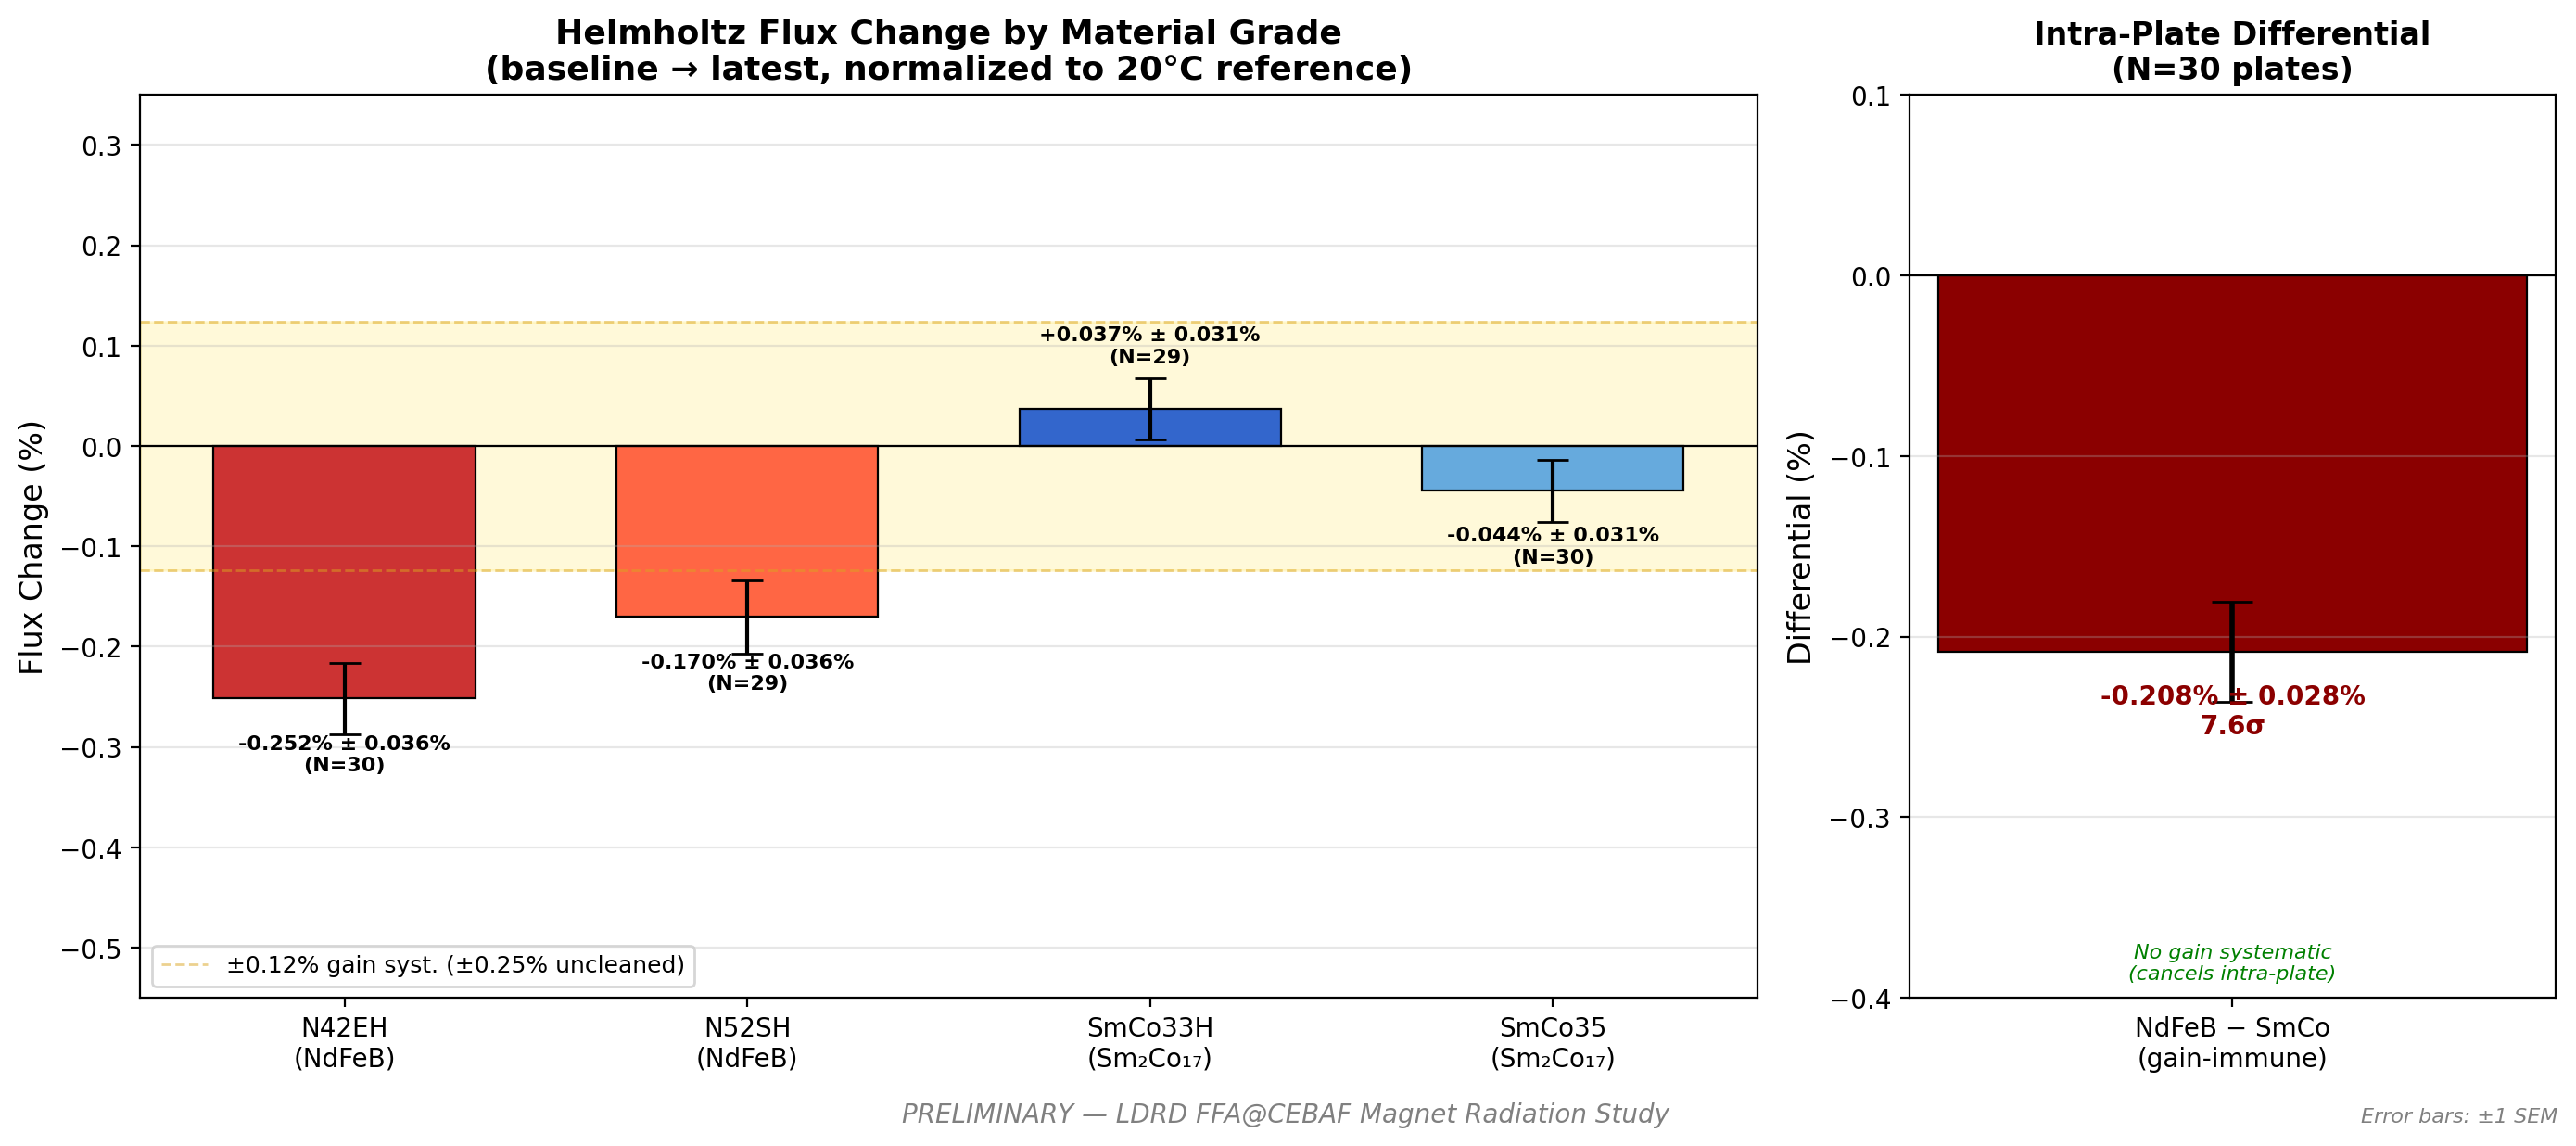
\includegraphics[width=0.95\textwidth]{figures/P1_material_comparison.png}
    \caption{\textbf{P1: Material comparison.} Percentage change from
    pre-deployment baseline for all four material grades on 30 tunnel Y-plates,
    temperature-normalized to the \SI{20}{\celsius} reference. Error bars show
    $\pm 1$~SEM. Both NdFeB grades (N42EH, N52SH) show significant negative
    changes (demagnetization), while both SmCo grades are consistent with zero,
    as expected for radiation-hard materials. The NdFeB--SmCo differential is
    $-0.208\% \pm 0.028\%$ ($7.6\sigma$).}
    \label{fig:P1}
\end{figure}

\subsection{Per-Material Results}
\label{sec:per_material}

Table~\ref{tab:per_material} shows the individual material results. The
systematic uncertainty of $\pm 0.124\%$ (gain drift) applies to each material
individually but \textbf{cancels} in the differential.

\begin{table}[H]
\centering
\caption{Per-material mean percentage changes for 30 tunnel Y-plates (v3
per-date temperature correction). Statistical uncertainties are SEM; systematic
uncertainty is from gain drift ($\pm 0.124\%$ cleaned).}
\label{tab:per_material}
\begin{tabular}{@{}lccccc@{}}
\toprule
\textbf{Material} & \textbf{Family} & \textbf{Mean $\Delta$ (\%)} &
\textbf{Stat.\ $\pm$ (\%)} & \textbf{Syst.\ $\pm$ (\%)} & \textbf{Note} \\
\midrule
N42EH  & NdFeB & $-0.252$ & 0.036 & 0.124 & Most degraded \\
N52SH  & NdFeB & $-0.170$ & 0.036 & 0.124 & Less degraded \\
SmCo33H & SmCo & $+0.037$ & 0.031 & 0.124 & Near zero \\
SmCo35  & SmCo & $-0.044$ & 0.031 & 0.124 & Near zero \\
\midrule
\textbf{NdFeB mean} & & $-0.211$ & 0.026 & 0.124 & \\
\textbf{SmCo mean}  & & $-0.004$ & 0.022 & 0.124 & \\
\textbf{Differential} & & $\mathbf{-0.208}$ & $\mathbf{0.028}$ & $\mathbf{0}$\footnotemark & \\
\bottomrule
\end{tabular}
\footnotetext{Gain systematic cancels by construction in the intra-plate
differential. The remaining systematics are $\pm 0.033\%$ (temperature) and
$\pm 0.014\%$ ($\alphar$ uncertainty).}
\end{table}

\textbf{Key observations:}
\begin{itemize}
    \item Both \ndfeb{} grades show clear demagnetization ($-0.252\%$ and
    $-0.170\%$), individually significant even with the gain systematic.
    \item Both \smco{} grades are consistent with zero ($+0.037\%$ and
    $-0.044\%$), as expected for radiation-hard materials.
    \item \textbf{N42EH degrades more than N52SH}. This is
    \textbf{inverted} from the thermal spike model prediction (which expects
    lower $\Hci$ = more vulnerable). This inversion is explained by dysprosium
    content: N42EH contains 1--2\,wt\%\,Dy while N52SH has zero
    (Section~\ref{sec:n42eh_inversion}).
\end{itemize}

\subsection{Lab Controls}
\label{sec:lab_controls}

Nine Y-plates stored in the laboratory with zero radiation exposure serve as
the control group:

\begin{table}[H]
\centering
\caption{Comparison of tunnel and lab Y-plate results. The lab differential is
consistent with zero, confirming no material-dependent measurement bias. The
tunnel--lab excess is independently significant at $4.3\sigma$.}
\label{tab:lab_controls}
\begin{tabular}{@{}lcccc@{}}
\toprule
& \textbf{NdFeB (\%)} & \textbf{SmCo (\%)} & \textbf{Differential (\%)} &
\textbf{Sig.} \\
\midrule
Tunnel (30 plates) & $-0.212 \pm 0.026$ & $-0.004 \pm 0.022$ & $-0.208 \pm 0.028$ & $7.6\sigma$ \\
Lab (9 plates) & $+0.014 \pm 0.025$ & $+0.020 \pm 0.018$ & $-0.007 \pm 0.038$ & $0.2\sigma$ \\
\textbf{Tunnel $-$ Lab} & $\mathbf{-0.226 \pm 0.036}$ & $-0.024 \pm 0.029$ & $\mathbf{-0.202 \pm 0.047}$ & $\mathbf{4.3\sigma}$ \\
\bottomrule
\end{tabular}
\end{table}

\begin{figure}[H]
    \centering
    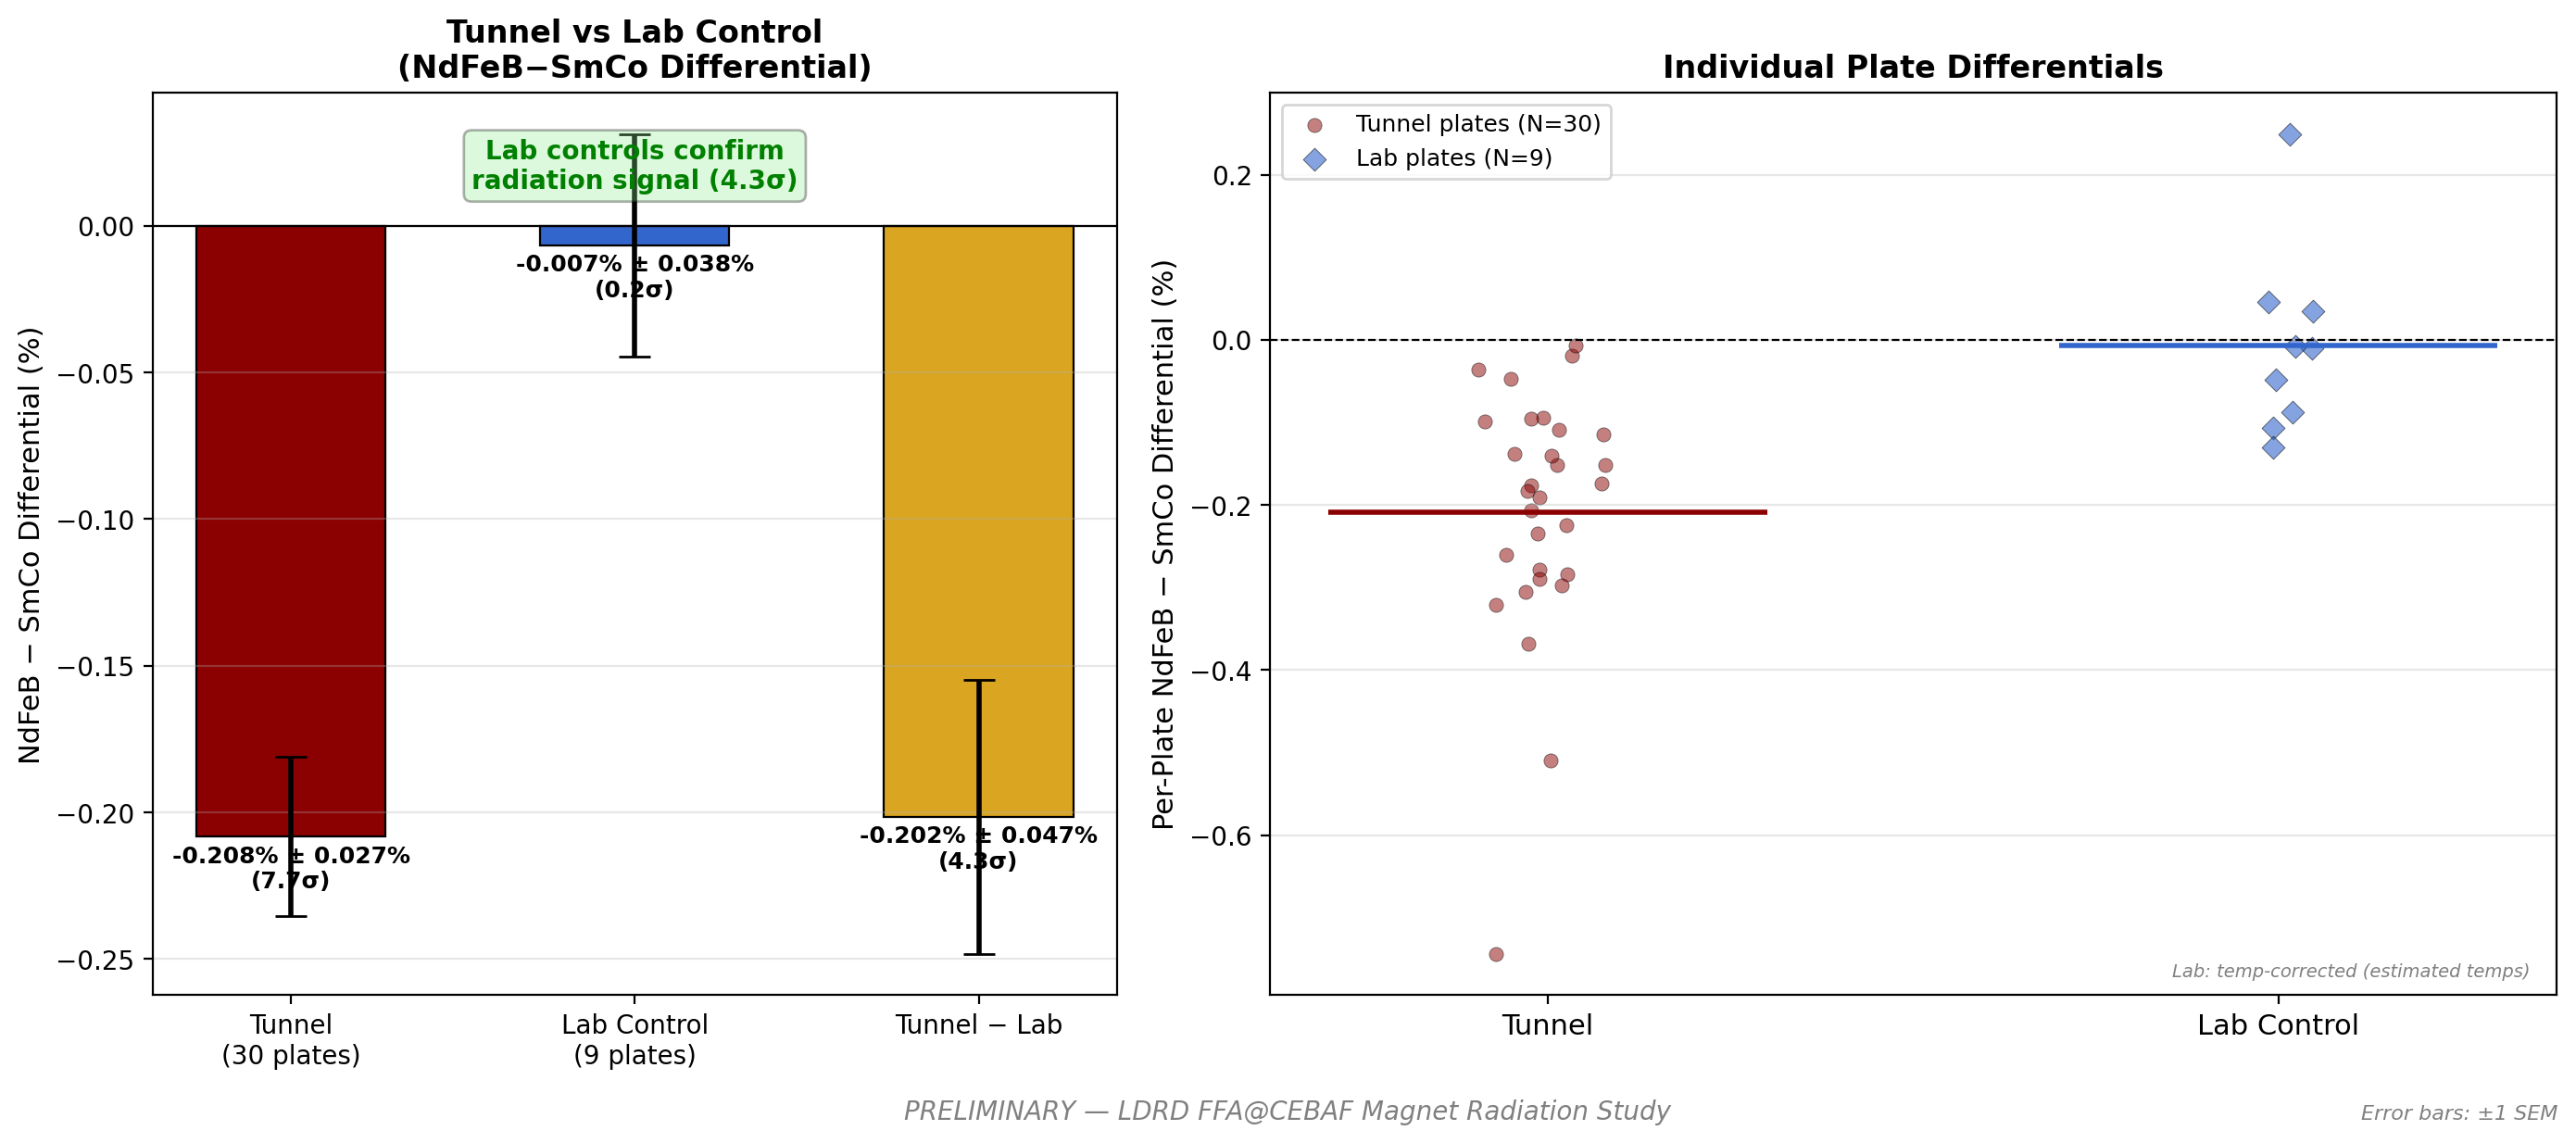
\includegraphics[width=0.95\textwidth]{figures/P4_lab_controls.png}
    \caption{\textbf{P4: Lab control comparison.} Material-by-material comparison
    of tunnel and lab Y-plates. Lab plates show no material-dependent effect,
    validating the measurement pipeline.}
    \label{fig:P4}
\end{figure}

The lab controls provide two critical validations:
\begin{enumerate}
    \item \textbf{Measurement system is unbiased}: The lab differential of
    $-0.007\% \pm 0.038\%$ ($0.2\sigma$) proves that the Helmholtz coil +
    temperature correction pipeline does not introduce a material-dependent
    artifact.
    \item \textbf{Independent confirmation}: The tunnel-minus-lab excess of
    $-0.202\% \pm 0.047\%$ ($4.3\sigma$) uses a completely different
    statistical test (two-population comparison) than the within-plate
    differential, and does not share the same systematic assumptions.
\end{enumerate}

\subsection{Regional Breakdown}

The degradation varies by tunnel location:

\begin{figure}[H]
    \centering
    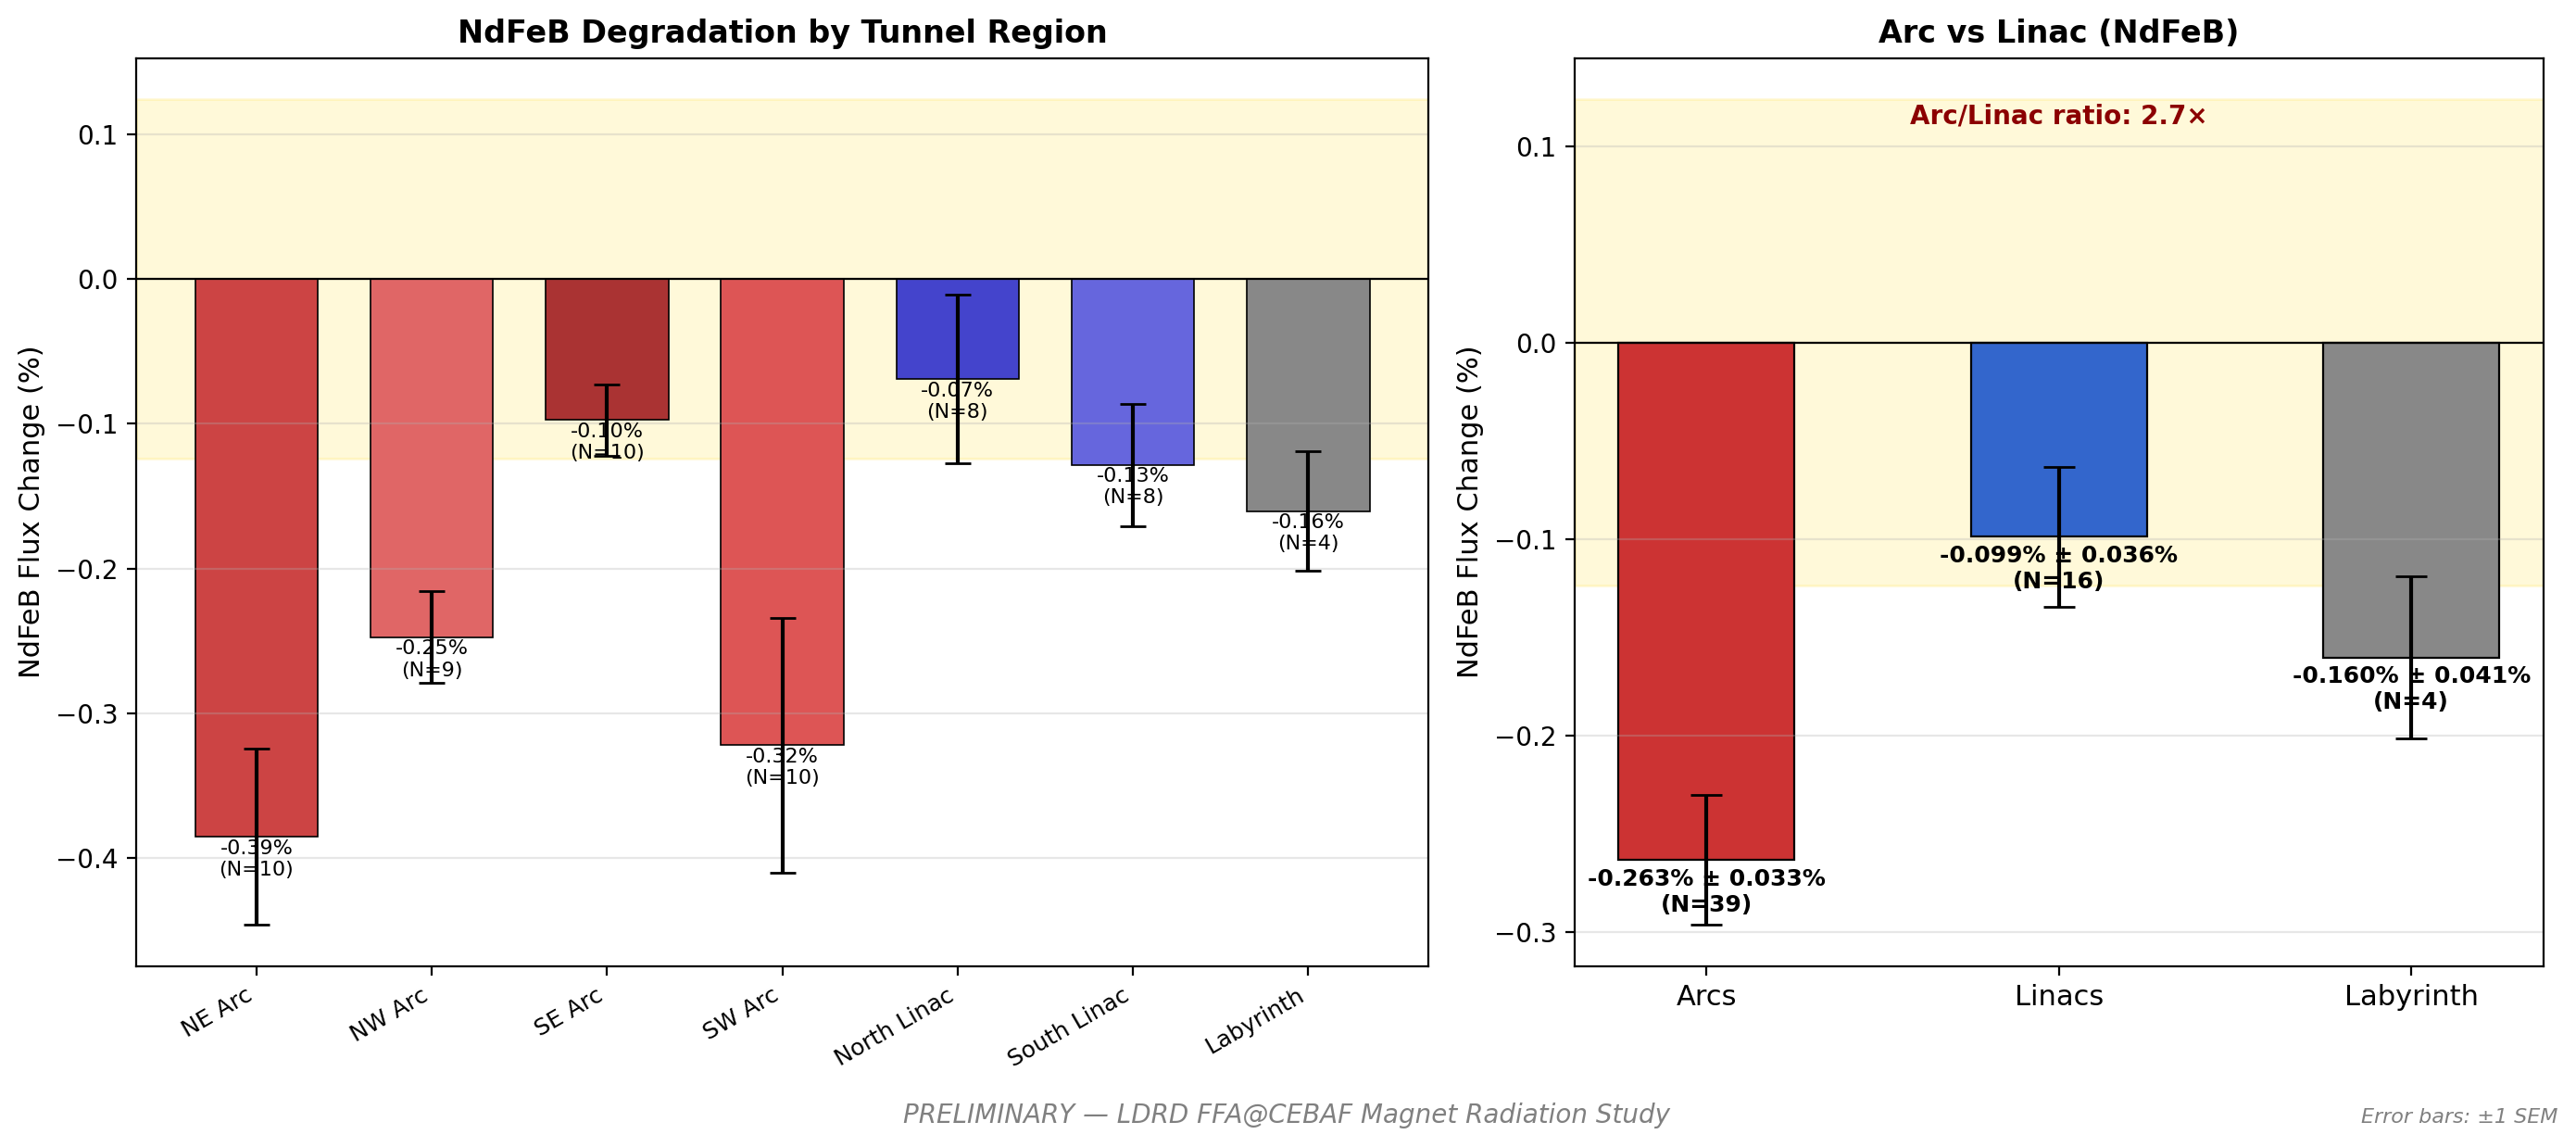
\includegraphics[width=0.95\textwidth]{figures/P3_regional_breakdown.png}
    \caption{\textbf{P3: Regional breakdown.} NdFeB--SmCo differential by
    accelerator region. Error bars show $\pm 1$~SEM. All regions show negative
    differentials (NdFeB degraded relative to SmCo), though with varying
    magnitudes reflecting the different radiation environments.}
    \label{fig:P3}
\end{figure}

\subsection{Time Series Evolution}

The degradation was tracked over multiple measurement campaigns:

\begin{figure}[H]
    \centering
    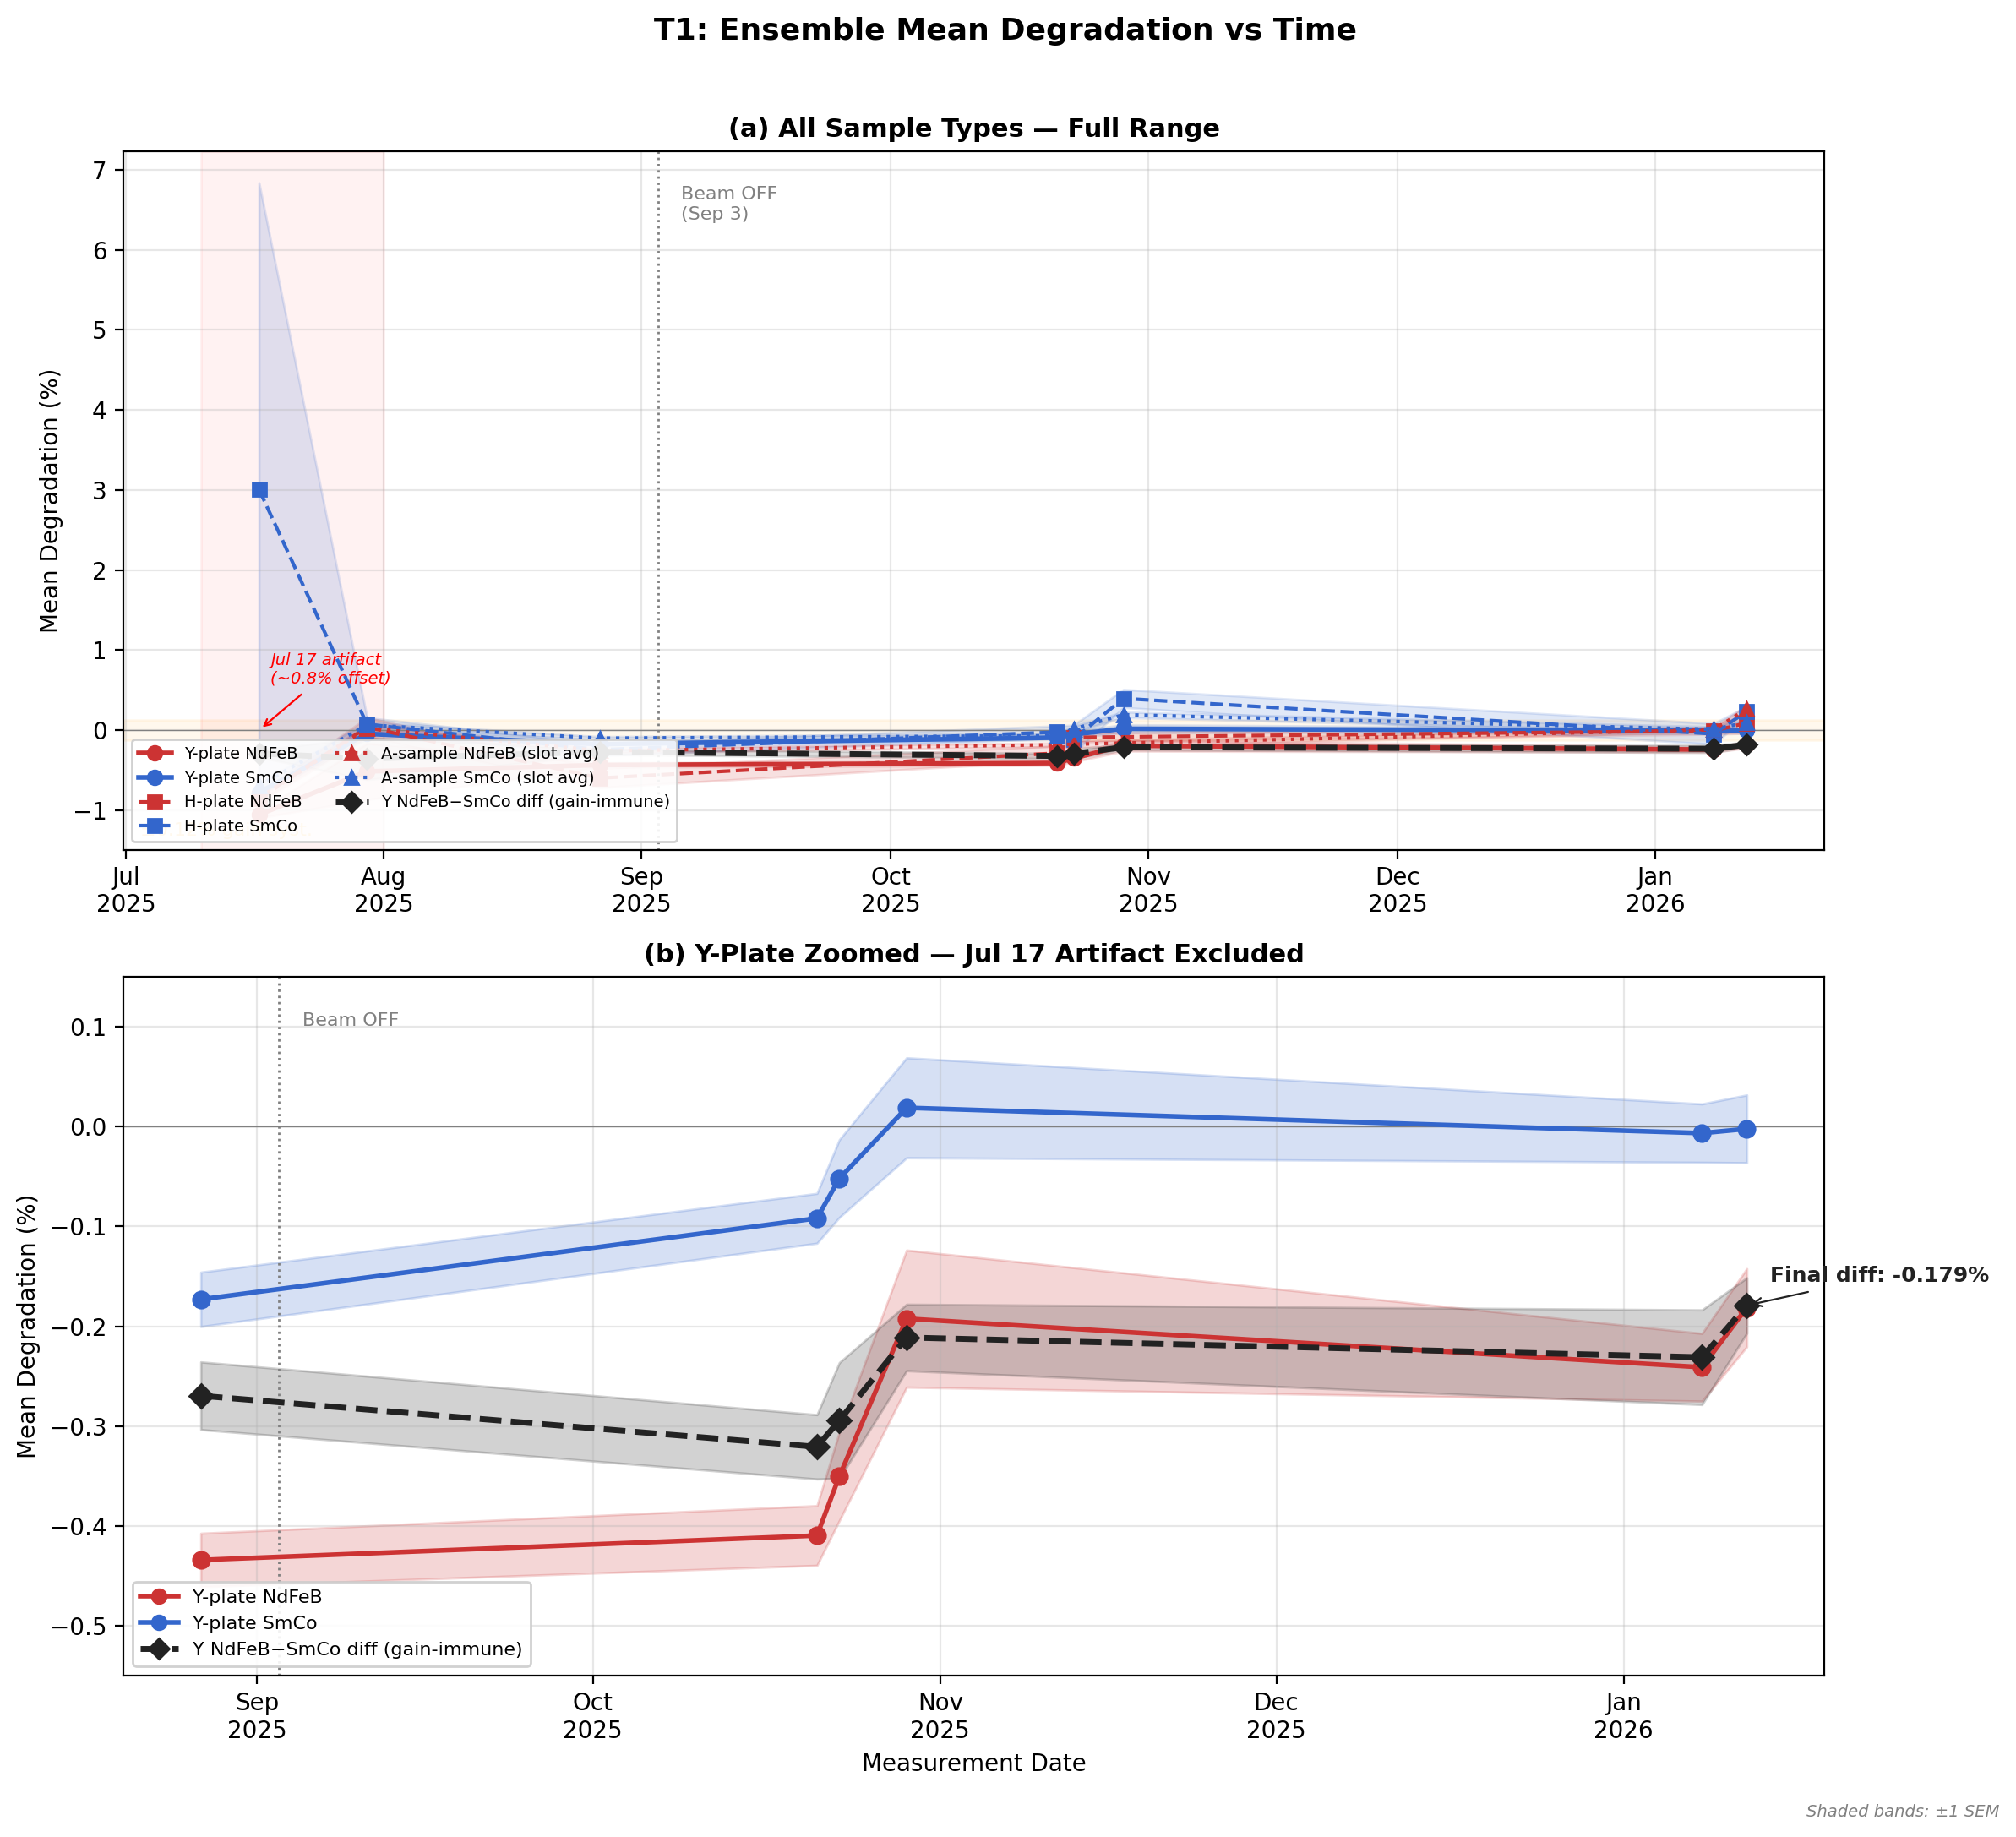
\includegraphics[width=0.95\textwidth]{figures/T1_ensemble_mean_vs_time.png}
    \caption{\textbf{T1: Ensemble mean vs.\ time.} (a)~Full view showing all
    material series and the Jul~17 artifact (first measurement session, only 15
    plates, likely coil warmup effect). (b)~Zoomed Y-plate view excluding the
    artifact, showing the NdFeB--SmCo differential stabilizing at $\sim
    -0.2\%$. The signal appears present from the first complete post-deployment
    measurement and remains roughly constant, consistent with damage occurring
    during the irradiation period, not progressive afterward. Shaded bands show
    $\pm 1$~SEM.}
    \label{fig:T1}
\end{figure}

\begin{figure}[H]
    \centering
    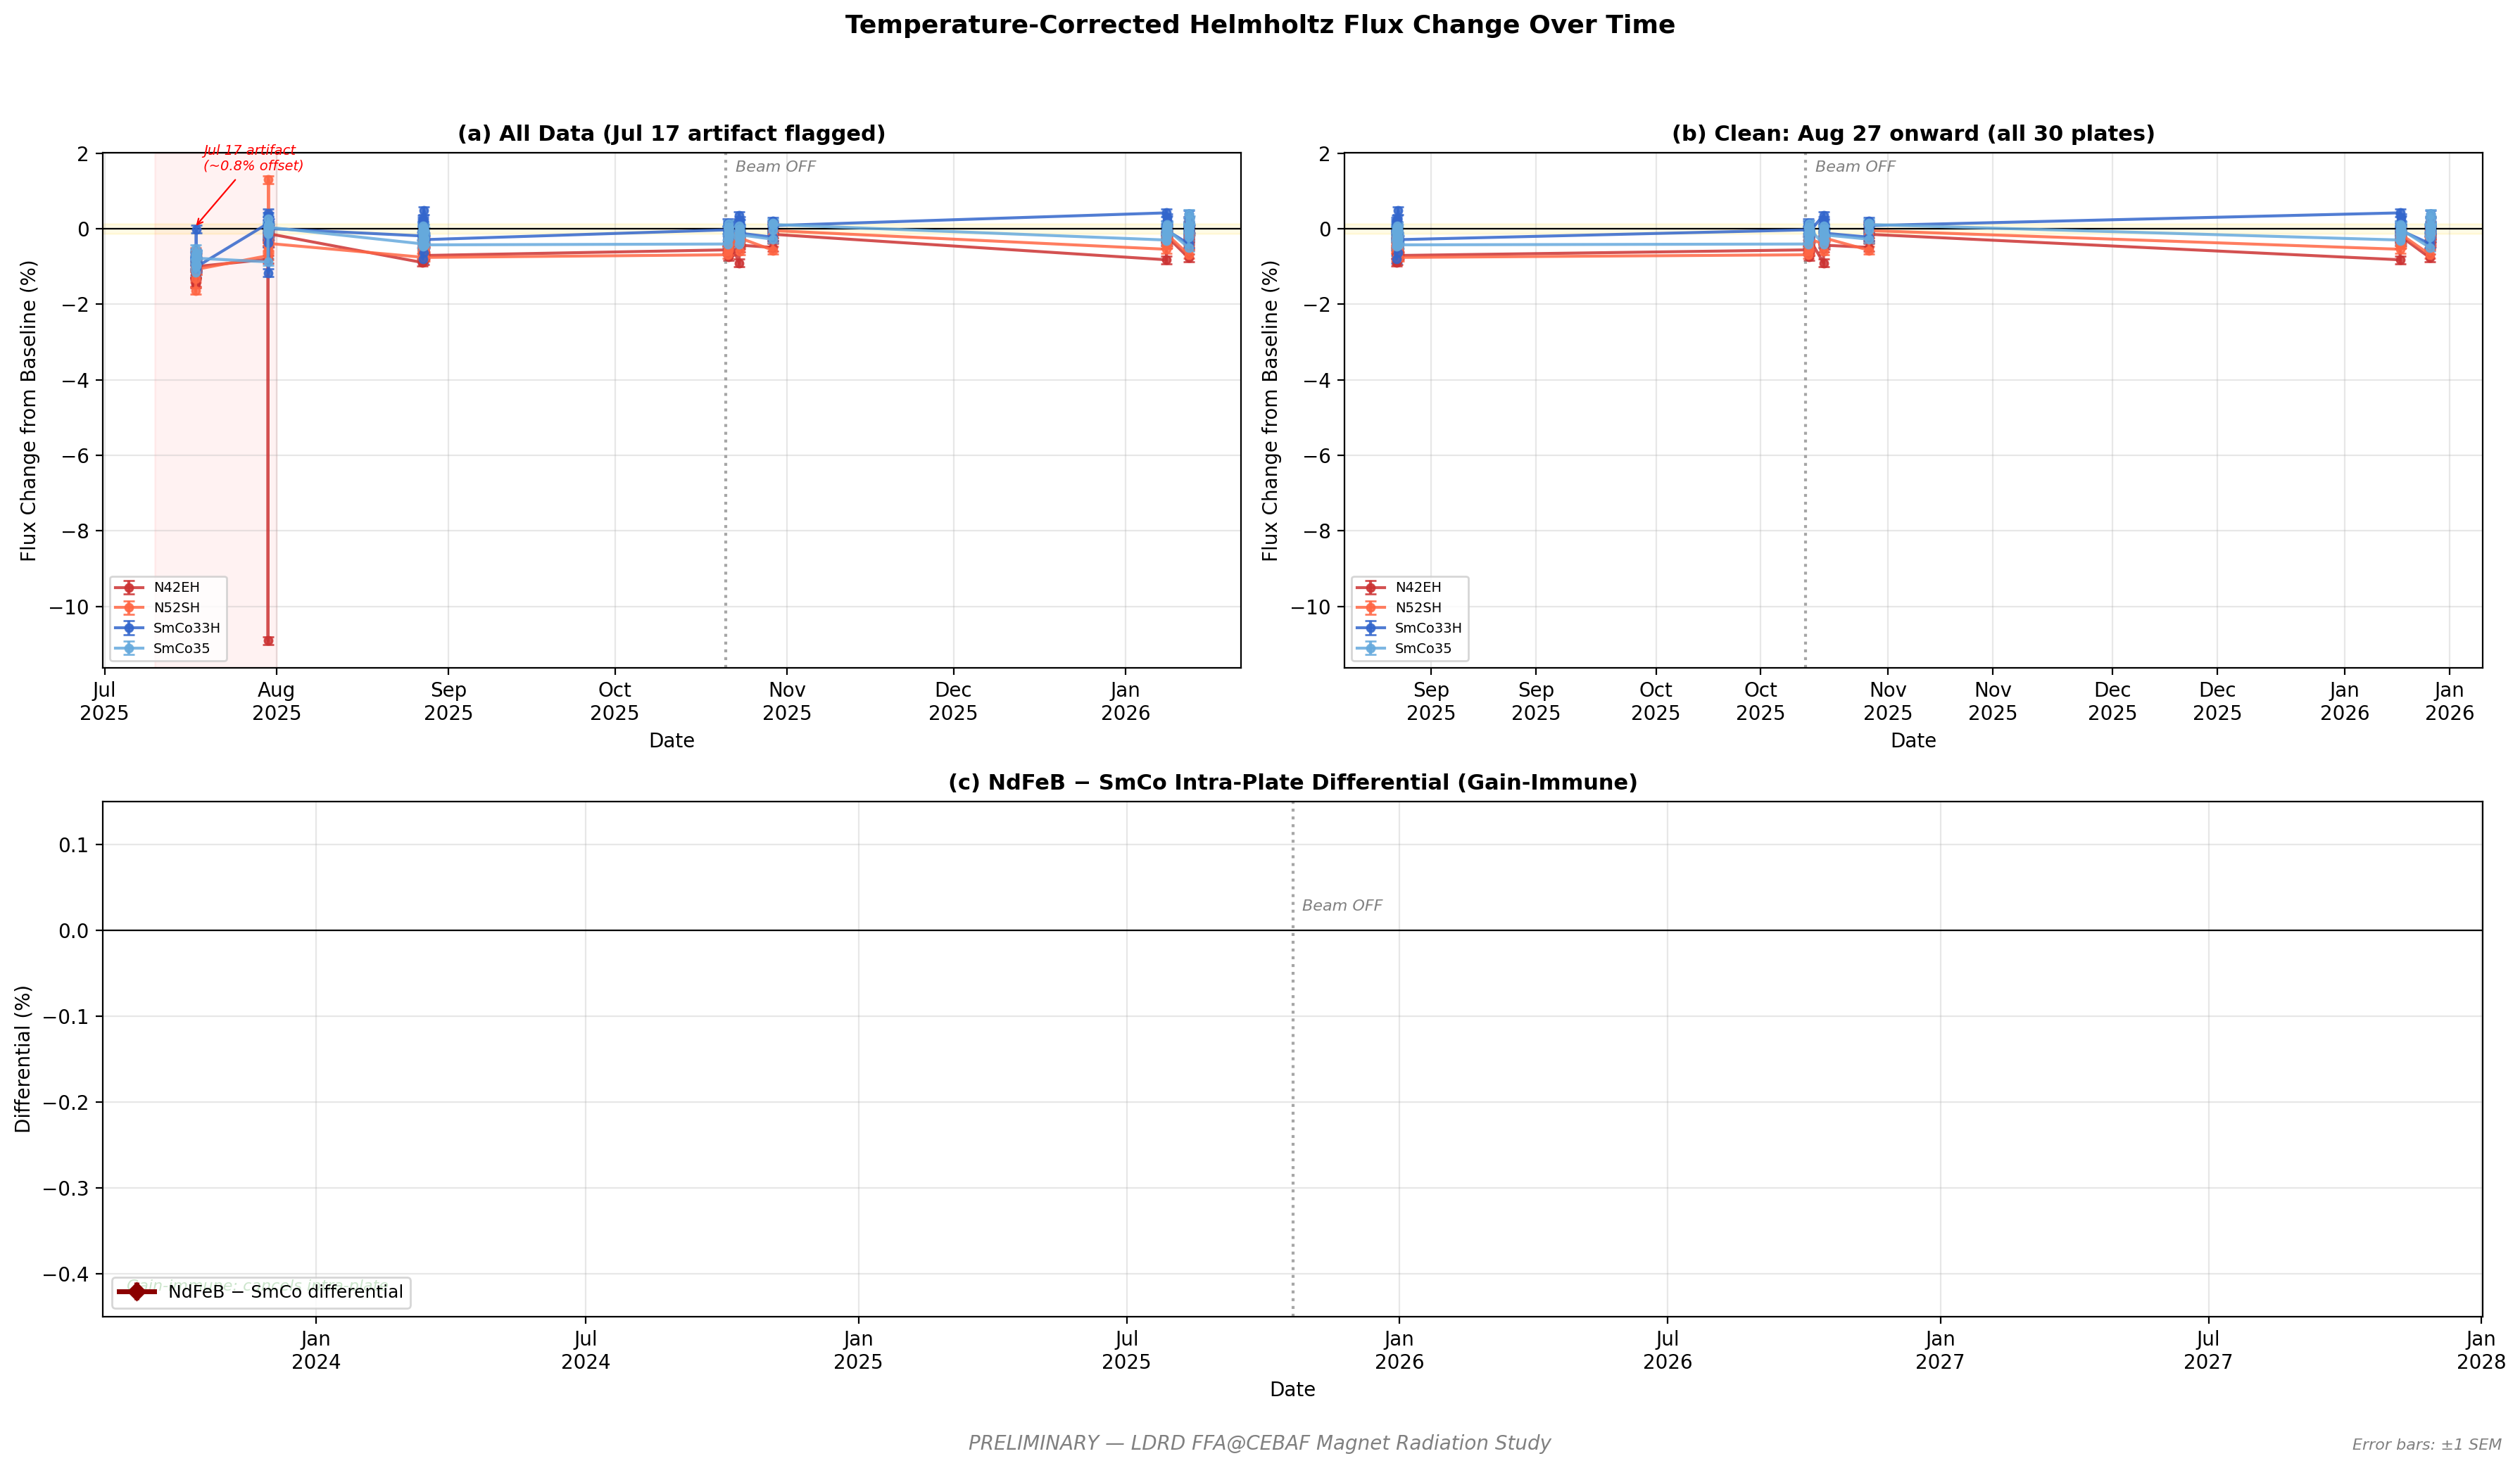
\includegraphics[width=0.95\textwidth]{figures/P2_timeseries_dual.png}
    \caption{\textbf{P2: Time series by material.} (a)~NdFeB grades over time.
    (b)~SmCo grades over time. (c)~NdFeB--SmCo differential time evolution
    computed per plate, with $\pm 1$~SEM bands and final value annotated. The
    differential is stable after the first complete measurement.}
    \label{fig:P2}
\end{figure}

\subsection{H-Plate and A-Sample Results}
\label{sec:ha_results}

H-plates and A-samples provide supplementary but noisier measurements:

\begin{table}[H]
\centering
\caption{Comparison of Y-plate, H-plate, and A-sample results. H-plates and
A-samples are \emph{not} gain-immune (inter-sample measurements) and have
fundamentally different systematics.}
\label{tab:sample_types}
\begin{tabular}{@{}lccccc@{}}
\toprule
\textbf{Type} & \textbf{Diff (\%)} & \textbf{SEM (\%)} & \textbf{Sig.} &
$N$ & \textbf{Method} \\
\midrule
\textbf{Y-plate} & $\mathbf{-0.208}$ & $\mathbf{0.028}$ & $\mathbf{7.6\sigma}$ & 30 plates & Intra-plate (gain-immune) \\
H-plate & $-0.122$ & 0.079 & $1.5\sigma$ & 37+48 pairs & Inter-sample \\
A-sample & $+0.020$ & 0.055 & $0.4\sigma$ & 13+16 slots & Inter-sample \\
\bottomrule
\end{tabular}
\end{table}

\textbf{Why H-plates and A-samples show weaker signals:}
\begin{enumerate}
    \item \textbf{Not gain-immune}: H and A measurements compare different
    plates/assemblies from different measurement sessions, carrying the full
    $\pm 0.124\%$ gain systematic.
    \item \textbf{Location confounding}: NdFeB H-plates (Hn) and SmCo H-plates
    (Hs) occupy different tunnel arcs, confounding material type with radiation
    environment.
    \item \textbf{Smaller $N$}: Fewer independent measurements than Y-plates.
\end{enumerate}

\textbf{Combining dilutes the signal.} Inverse-variance weighted combination
of Y+H+A NdFeB means drops significance from $8.2\sigma$ to $5.3\sigma$,
because H/A means near zero pull the average toward zero. The Y-plate
differential is always the headline result.

\textbf{Halbach proxy potential.} Although current H/A data cannot resolve
configuration-dependent differences (due to single-reading baselines, gain
systematics, and location confounding), the H-plate configurations were
designed as Halbach array proxies. If baseline issues are resolved (e.g.,
through Honeywell temperature data or multi-point baselines in a second
exposure campaign), comparing Alpha (aligned), Beta (antiparallel), and
Gamma (perpendicular) configurations could directly reveal whether field
alignment relative to neighbors affects the degradation rate. This would be a critical input for Halbach magnet design
decisions~\cite{NGotta2024}. The A-samples within each H-plate provide
additional granularity for this comparison.

\begin{figure}[H]
    \centering
    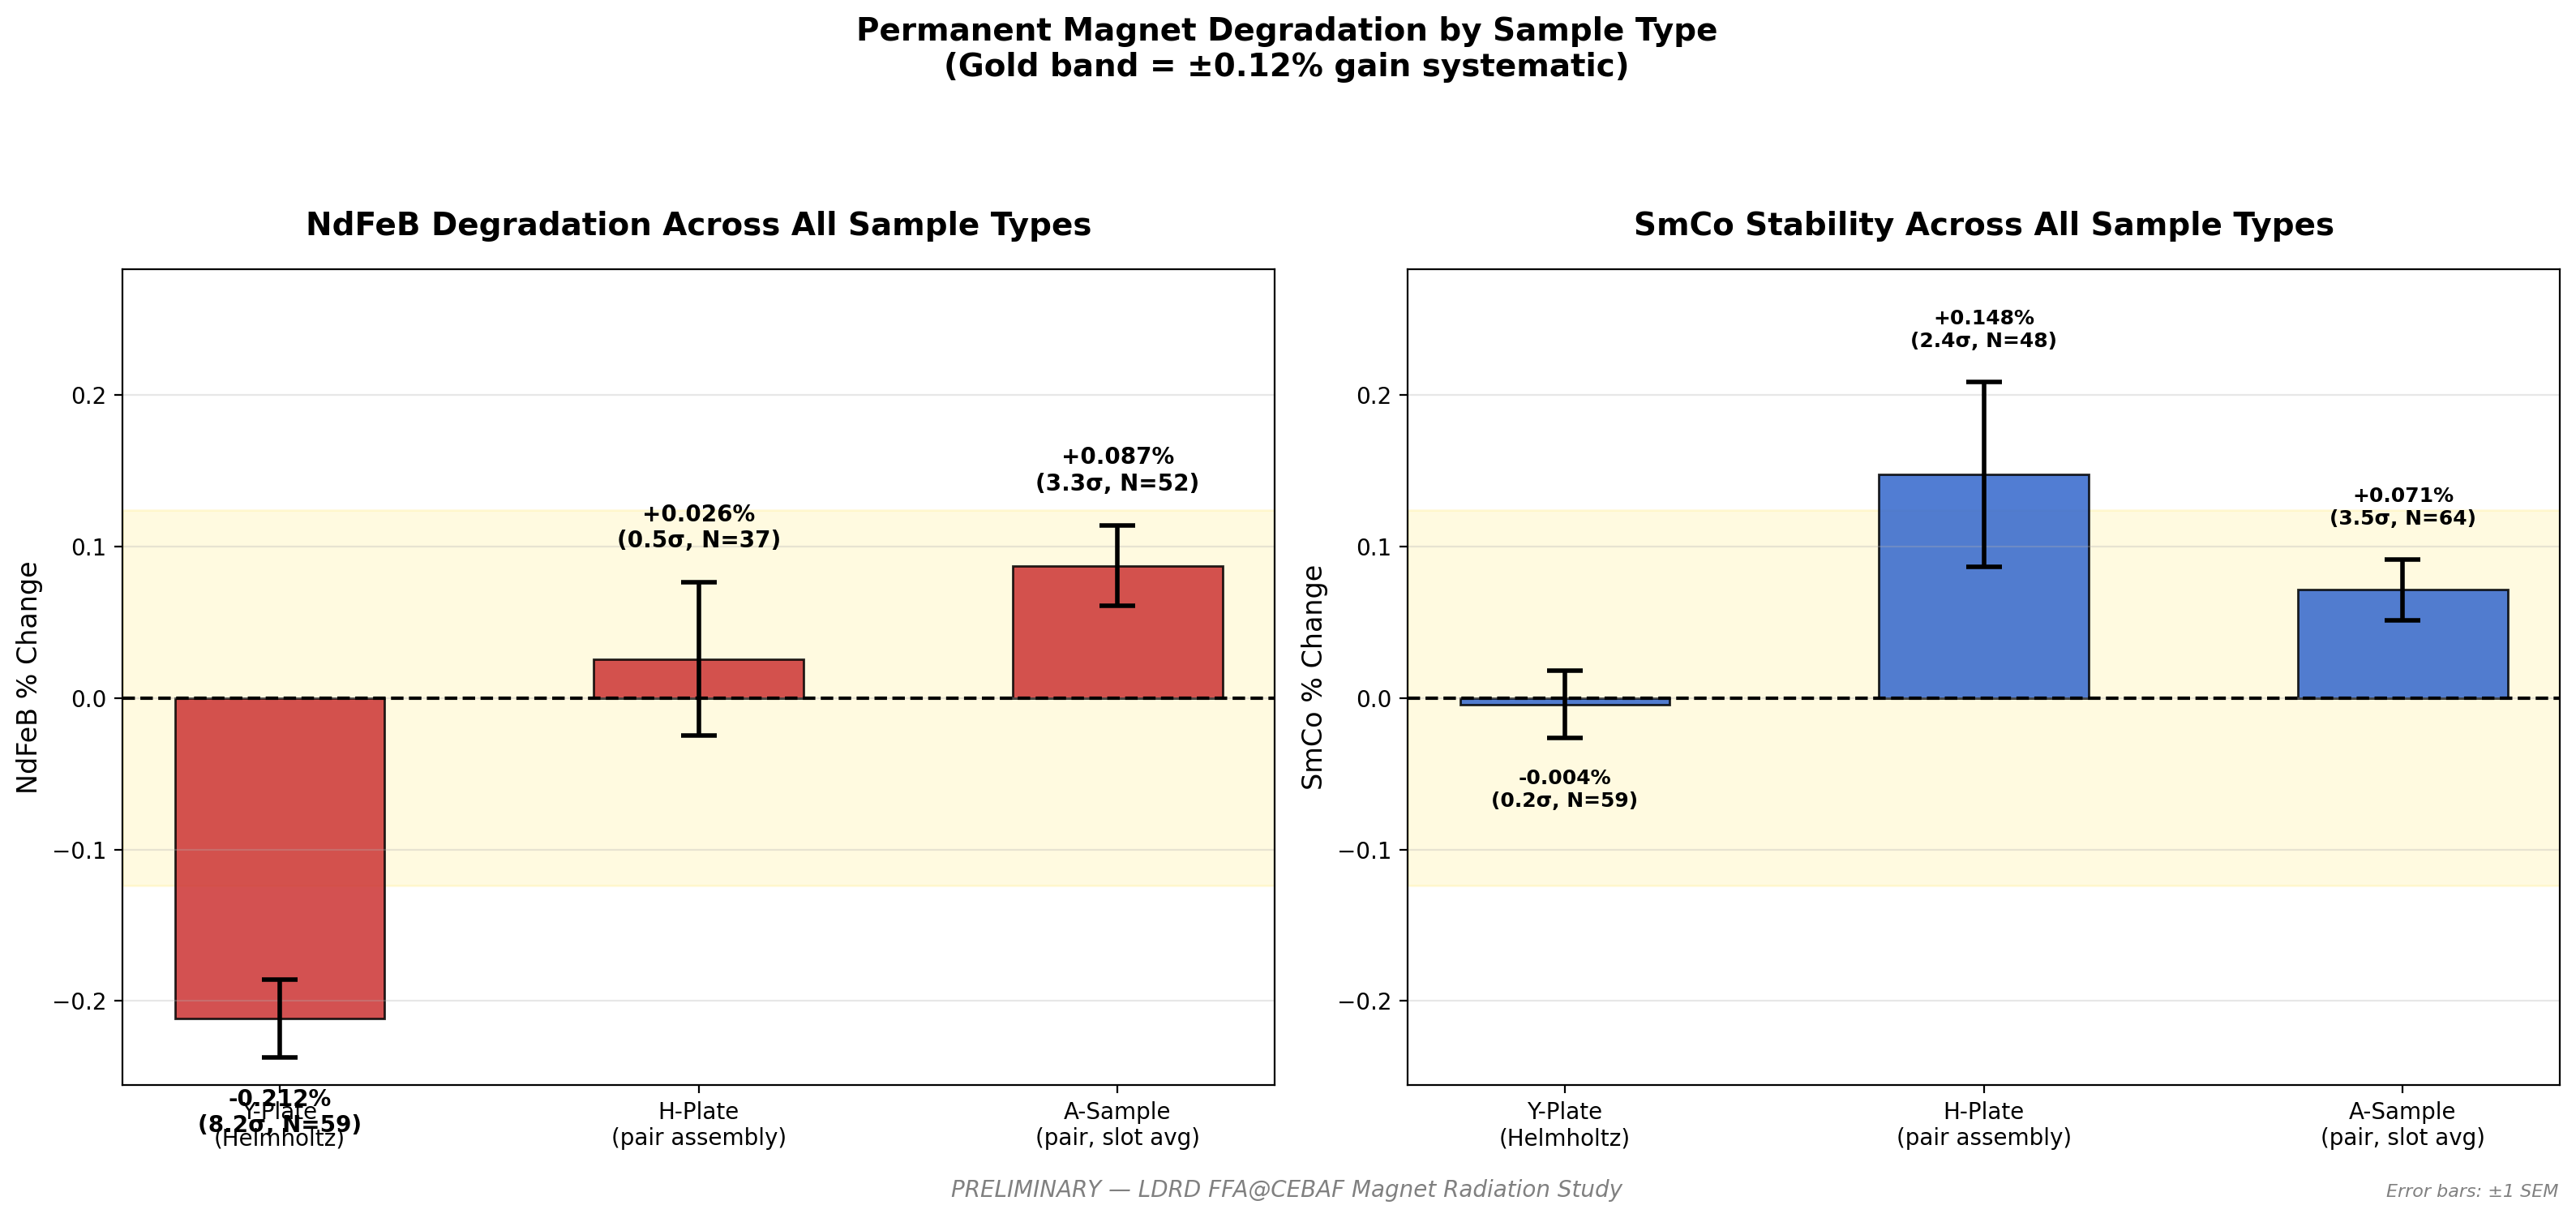
\includegraphics[width=0.95\textwidth]{figures/P12_combined_YHA.png}
    \caption{\textbf{P12: Combined Y/H/A comparison.} All three sample types
    shown together. The Y-plate differential is the most precise and shows the
    clearest signal.}
    \label{fig:P12}
\end{figure}

\subsection{Gain Drift Systematic}
\label{sec:gain_systematic}

The Helmholtz coil gain drift is quantified from the
\texttt{gain\_systematic\_analysis.py} script:

\begin{itemize}
    \item \textbf{Session-to-session drift}: 0.5--0.7\% typical
    \item \textbf{Cleaned gain systematic}: $\pm 0.124\%$ (after removing two
    outliers: Y-34-4 and Y-40-4, which showed $>$3\% changes due to known
    baseline issues)
    \item \textbf{Uncleaned}: $\pm 0.248\%$
\end{itemize}

Known artifacts:
\begin{itemize}
    \item \textbf{Oct 21, 2025}: $\sim$0.3\% thermal lag artifact during a
    beam-off period (tunnel cooling). Common-mode, affects all materials equally.
    \item \textbf{Jul 17, 2025}: $\sim$0.8\% offset in the first tunnel
    measurement (only 15 plates). Likely coil warmup or connection effects.
    Superseded by later full surveys.
\end{itemize}

% ============================================================================
\section{Dose--Degradation Correlations}
\label{sec:dose_degradation}
% ============================================================================

\subsection{Gamma Dose Does NOT Correlate with Degradation}

This is one of the most important findings in the study. Despite gamma doses
spanning five orders of magnitude (\SIrange{0.3}{23451}{Gy}), there is
\textbf{no correlation} between gamma dose and degradation:

\begin{table}[H]
\centering
\caption{Spearman rank correlations between dose types and degradation metrics.
Significant correlations ($p < 0.05$) are shown in bold.}
\label{tab:correlations}
\begin{tabular}{@{}lccc@{}}
\toprule
\textbf{Dose Type} & \textbf{Metric} & $\rho$ & $p$ \\
\midrule
\multirow{3}{*}{Gamma (AIdata)} & NdFeB mean & $+0.270$ & 0.15 \\
 & SmCo mean & $+0.125$ & 0.51 \\
 & Differential & $+0.210$ & 0.27 \\
\midrule
\multirow{3}{*}{\textbf{Neutron (CR-39)}} & \textbf{NdFeB mean} & $\mathbf{+0.459}$ & $\mathbf{0.011}$ \\
 & SmCo mean & $+0.075$ & 0.69 \\
 & \textbf{Differential} & $\mathbf{+0.389}$ & $\mathbf{0.034}$ \\
\bottomrule
\end{tabular}
\end{table}

\textbf{Why we use Spearman rather than Pearson}: The Spearman rank correlation
is a non-parametric measure of monotonic association. It does not assume a
linear relationship or normally distributed variables. This is appropriate here
because:
\begin{itemize}
    \item Dose spans five orders of magnitude (highly non-normal)
    \item The dose--response relationship, if it exists, may not be linear
    \item The degradation data contains outliers (e.g., Y-34-4, Y-40-4)
    \item With $N = 30$, parametric assumptions are difficult to verify
\end{itemize}

The Spearman $\rho$ ranges from $-1$ (perfect inverse monotonic relationship)
to $+1$ (perfect positive). The $p$-value tests the null hypothesis that $\rho
= 0$ (no monotonic association). Our $\rho = 0.210$, $p = 0.27$ for
gamma-differential means there is no evidence for a monotonic relationship
between gamma dose and the NdFeB--SmCo degradation differential.

\begin{figure}[H]
    \centering
    
\includegraphics[width=0.95\textwidth]{figures/rod_correlation_R1_side_by_side.png}
    \caption{\textbf{R1: Dose vs.\ degradation side-by-side.} Left: gamma dose
    (Gy) vs.\ NdFeB mean degradation. Right: neutron dose (rem) vs.\ NdFeB
    mean degradation. The gamma plot shows no trend; the neutron plot shows a
    marginal positive correlation. Error bars: $x =$ dose $\sigma$, $y = \pm
    1$~SEM.}
    \label{fig:R1}
\end{figure}

\subsection{Neutron Dose Shows Significant Correlation}

In contrast to gamma, the neutron dose (from CR-39 track-etch detectors) shows
a \textbf{significant} correlation with degradation:
\begin{itemize}
    \item NdFeB mean: $\rho = +0.459$, $p = 0.011$ (significant)
    \item Differential: $\rho = +0.389$, $p = 0.034$ (significant)
    \item SmCo: $\rho = +0.075$, $p = 0.69$ (null, as expected)
\end{itemize}

The SmCo null is physically meaningful: radiation-hard \smco{} shows no
dose-dependent degradation, while radiation-sensitive \ndfeb{} does. This
material selectivity is exactly what the damage mechanism predicts.

\begin{figure}[H]
    \centering
    
\includegraphics[width=0.95\textwidth]{figures/rod_correlation_R2_by_material.png}
    \caption{\textbf{R2: Dose--degradation by material.} Correlations shown
    separately for each material grade. NdFeB grades (left panels) show
    negative trends with dose; SmCo grades (right panels) show no trend.}
    \label{fig:R2}
\end{figure}

\begin{figure}[H]
    \centering
    
\includegraphics[width=0.95\textwidth]{figures/rod_correlation_R3_differential.png}
    \caption{\textbf{R3: Differential vs.\ dose.} The gain-immune NdFeB--SmCo
    differential plotted against gamma and neutron dose, with Spearman
    correlations annotated.}
    \label{fig:R3}
\end{figure}

\subsection{Gamma Null as a Positive Finding}
\label{sec:gamma_null}

The absence of gamma dose correlation is not a weakness; it is a
\textbf{physically meaningful result}:

\begin{itemize}
    \item \textbf{Alderman et al.}~\cite{Alderman} irradiated NdFeB with pure
    gamma radiation (\SI{60}{Co} equivalent) up to \SI{7}{MGy} (700~Mrad) and
    observed \textbf{no measurable demagnetization}. This is the highest-dose
    gamma-only null in the literature.
    \item Our maximum gamma dose (\SI{23451}{Gy} at Y-22) is
    \textbf{$\sim$300$\times$ below} the Alderman null threshold.
    \item The gamma null is therefore exactly what the literature predicts at
    these dose levels.
\end{itemize}

Combined with the significant neutron correlation, this provides the
\textbf{first in-situ accelerator confirmation} of the neutron $\gg$ gamma
damage hierarchy established by controlled irradiation
experiments~\cite{Shen2018,Alderman,APSLS290}.

\subsection{Fast vs.\ Thermal Neutron Correlations}
\label{sec:fast_thermal}

The CR-39 track-etch detectors provide separate thermal and fast neutron
doses. This distinction is critical for mechanism identification:
\begin{itemize}
    \item \textbf{Thermal neutrons} damage magnets primarily via nuclear
    capture reactions, especially ${}^{10}$B(n,$\alpha$)${}^{7}$Li ($\sigma =
    \SI{3840}{barns}$, $Q = \SI{2.3}{MeV}$). The alpha particle and lithium
    ion create localized ionization tracks that can disrupt grain boundary
    phases.
    \item \textbf{Fast neutrons} damage via displacement cascades: the primary
    knock-on atom (PKA) displaces lattice atoms, creating a nanoscale region
    of disorder. If the local temperature exceeds $\Tc$, irreversible domain
    reversal can occur (the thermal spike mechanism).
\end{itemize}

\begin{table}[H]
\centering
\caption{Fast vs.\ thermal neutron correlations with degradation. Total neutron
(fast $+$ thermal) produces the strongest correlation because it combines
independent dose information and reduces measurement noise. Neither component
individually reaches $p < 0.05$ for the differential.}
\label{tab:fast_thermal}
\begin{tabular}{@{}lcccc@{}}
\toprule
\textbf{Neutron Type} & \multicolumn{2}{c}{\textbf{NdFeB mean}} &
\multicolumn{2}{c}{\textbf{Differential}} \\
& $\rho$ & $p$ & $\rho$ & $p$ \\
\midrule
Fast   & $+0.308$ & 0.10 & $+0.215$ & 0.26 \\
Thermal & $+0.187$ & 0.33 & $+0.151$ & 0.43 \\
\textbf{Total} & $\mathbf{+0.459}$ & $\mathbf{0.011}$ & $\mathbf{+0.389}$ & $\mathbf{0.034}$ \\
\bottomrule
\end{tabular}
\end{table}

\textbf{Key finding}: Fast neutron dose correlates more strongly than thermal
($\rho = 0.308$ vs.\ $0.187$ for NdFeB; $\rho = 0.215$ vs.\ $0.151$ for
differential), suggesting displacement cascades as the dominant damage
mechanism rather than nuclear capture. However, neither component individually
reaches significance; the total neutron sum produces the strongest correlation
by combining independent dose information. The median fast/thermal ratio at
\CEBAF is 12.5 (range 9--16), confirming that fast neutrons dominate the
spectrum.

\begin{figure}[H]
    \centering
    
\includegraphics[width=0.95\textwidth]{figures/rod_correlation_R6_fast_thermal_neutron.png}
    \caption{\textbf{R6: Fast vs.\ thermal neutron correlations.} $2\times 3$
    grid (rows = fast/thermal, columns = NdFeB/SmCo/differential) with Spearman
    correlations and linear fit lines. Fast neutrons show stronger correlations
    than thermal, pointing to displacement cascades as the dominant damage
    mechanism.}
    \label{fig:R6}
\end{figure}

\subsection{Multiple Comparisons Context}
\label{sec:multiple_comparisons}

The analysis tests correlations for 7 degradation metrics $\times$ 3 dose
types = 21 hypothesis tests. The neutron-differential $p = 0.03$ would
\textbf{not survive} a Bonferroni correction (threshold $= 0.05/21 = 0.0024$).

However, this test is properly framed as a \textit{directed hypothesis test},
not exploratory data mining:
\begin{enumerate}
    \item The radiation damage hierarchy (neutron $\gg$ gamma) is
    well-established in the literature \cite{Shen2018,Simos2018,Bizen2016}.
    \item The NdFeB-specific effect (SmCo null) is consistent with the known
    Curie temperature difference.
    \item The gamma null matches the Alderman et al.~\cite{Alderman} result at \SI{7}{MGy}.
    \item The fast $>$ thermal trend matches the displacement cascade mechanism
    expected at accelerator neutron energies.
\end{enumerate}

We report uncorrected $p$-values throughout and note that a Bonferroni
correction would render individual results non-significant at the 5\% level.

\subsection{Dose--Position Inversion}
\label{sec:position_inversion}

The most striking spatial pattern in this study is a \textbf{dose--position
inversion} in the arc stacks: degradation increases monotonically from the
bottom to the top of each stack, while the measured gamma dose follows the
\emph{opposite} trend.

\begin{table}[H]
\centering
\caption{Mean degradation and dose by arc line position ($N = 20$ arc plates,
4 per line). Line~1 (top) shows the most degradation but the least dose.}
\label{tab:line_inversion}
\begin{tabular}{@{}ccccc@{}}
\toprule
\textbf{Line (arc)} & $N$ & \textbf{Mean Diff (\%)} &
\textbf{Mean Gamma (Gy)} & \textbf{Mean Neutron (rem)} \\
\midrule
Line 1 (top)   & 4 & $-0.431$ & 30    & 17  \\
Line 2         & 4 & $-0.258$ & 320   & 21  \\
Line 3         & 4 & $-0.176$ & 652   & 838 \\
Line 4         & 4 & $-0.133$ & 1,119 & 388 \\
Line 5 (bottom)& 4 & $-0.142$ & 668   & 16  \\
\bottomrule
\end{tabular}
\end{table}

Spearman correlations for arc plates ($N = 20$):
\begin{itemize}
    \item Line vs.\ differential: $\rho = +0.601$ ($p = 0.005$), \textbf{highly significant}
    \item Line vs.\ gamma dose: $\rho = +0.515$ ($p = 0.02$); dose increases downward
    \item Line vs.\ neutron dose: $\rho = -0.043$ ($p = 0.86$); no line trend
\end{itemize}

\begin{figure}[H]
    \centering
    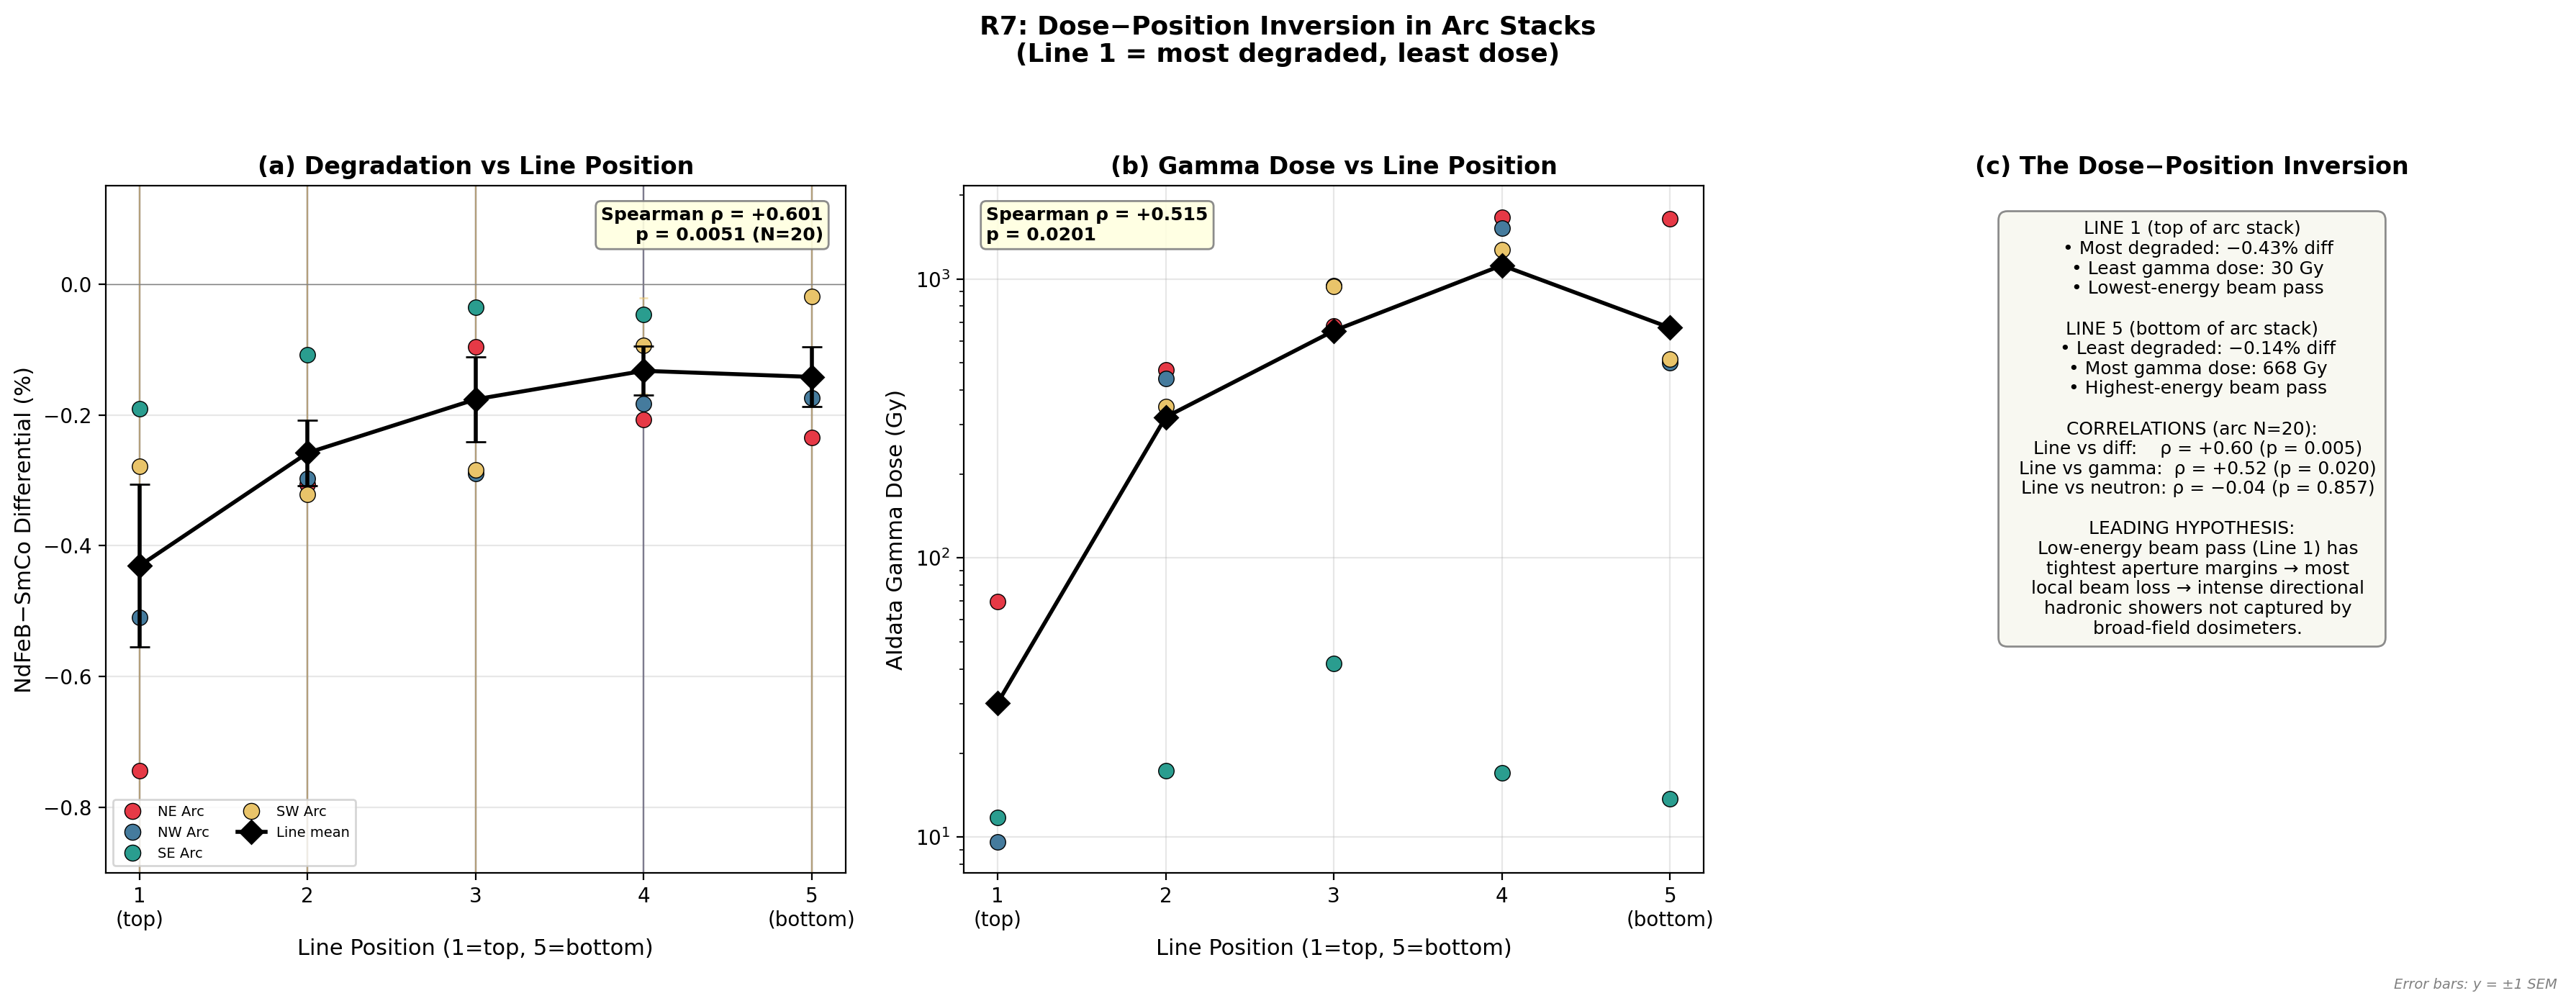
\includegraphics[width=0.95\textwidth]{figures/rod_correlation_R7_line_position_inversion.png}
    \caption{\textbf{R7: Dose--position inversion.} Three-panel figure showing
    (a)~degradation vs.\ line position by arc, (b)~gamma dose vs.\ line
    position, (c)~summary with leading hypothesis. The monotonic trend of
    increasing degradation toward Line~1 is opposite to the measured dose
    gradient.}
    \label{fig:R7}
\end{figure}

This inversion (more degradation where there is less measured dose) requires
explanation. We consider four hypotheses:

\paragraph{Hypothesis~1: Beam pass structure and local beam loss (leading).}
In \CEBAF's recirculating arcs, each line position corresponds to a different
beam energy pass. Line~1 (top) carries the lowest-energy beam, which has the
lowest magnetic rigidity and therefore the \textbf{largest beam envelope and
highest probability of beam loss} at aperture restrictions. Local beam losses
at nearby magnets produce intense, directional hadronic showers (neutrons +
charged secondaries) that may not be uniformly sampled by the co-located rod
dosimeters, which measure the broad ambient radiation field integrated over
the wear period.

\paragraph{Hypothesis~2: Neutron spectrum hardness.}
Even at the same measured neutron dose (in rem, a quality-weighted unit),
harder neutrons produce more displacement damage per unit dose. Line~1 may see
a harder neutron spectrum from direct hadronic cascades, while lower lines
receive more moderated neutrons that register higher dose but cause less
damage per unit.

\paragraph{Hypothesis~3: Solid angle and secondary geometry.}
Line~1 (top) has maximum exposure to the upper hemisphere where beam pipe
radiation originates. Lower lines are partially shielded by plates and
hardware above them. The dosimeters may not capture this shielding asymmetry.

\paragraph{Hypothesis~4: Vibration and mechanical effects.}
The top position may experience more vibration from nearby magnets during
beam operations. However, this is unlikely to produce a permanent
demagnetization mimicking the NdFeB-selective, SmCo-null pattern.

\textbf{Assessment}: Hypothesis~1 is the most physically plausible. \CEBAF
beam loss distributions are well-known to be highly non-uniform, concentrated
at specific lattice elements. The lowest-energy pass traverses the innermost
orbit with the tightest aperture margins. A Monte Carlo simulation (e.g.,
BDSIM/GEANT4) would directly test this hypothesis (Section~\ref{sec:future}).

\textbf{Key point}: The dose--position inversion does not undermine the
radiation damage interpretation. It suggests that the damage-causing radiation
(likely hadronic secondaries from beam loss) is \emph{not proportional} to the
broad ambient dose field. The significant neutron correlation ($\rho = 0.389$,
$p = 0.03$), the NdFeB-selective/SmCo-null material dependence, and the lab
control null result all independently confirm radiation-induced degradation.

% ============================================================================
\section{Systematic Error Analysis and Uncertainty Budget}
\label{sec:systematics}
% ============================================================================

This section brings together all identified sources of systematic uncertainty,
organized from largest to smallest impact.

\subsection{Formal Error Budget: Gain-Immune Differential}

The headline result uses the gain-immune intra-plate differential, for which
the dominant Helmholtz gain systematic \textbf{cancels by construction}
(Section~\ref{sec:gain_immune}). The remaining uncertainties are:

\begin{table}[H]
\centering
\caption{Formal error budget for the NdFeB--SmCo differential. The combined
uncertainty is computed in quadrature.}
\label{tab:error_budget}
\begin{tabular}{@{}lcl@{}}
\toprule
\textbf{Source} & \textbf{Magnitude (\%)} & \textbf{Notes} \\
\midrule
Statistical (SEM, 30 plates) & $\pm 0.028$ & From data \\
Baseline temperature ($\pm$\SI{0.5}{\celsius}) & $\pm 0.033$ & $0.066\%/\si{\celsius} \times 0.5$ \\
$\alphar$ uncertainty ($\pm$10\%) & $\pm 0.014$ & Manufacturer tolerance \\
Gain systematic & \textbf{0 (cancels)} & Intra-plate by construction \\
\midrule
\textbf{Combined (quadrature)} & $\pm 0.045$ & $\sqrt{0.028^2 + 0.033^2 + 0.014^2}$ \\
\midrule\midrule
\textbf{Result} & \multicolumn{2}{l}{$\mathbf{-0.208\% \pm 0.045\%}$ ($4.6\sigma$ combined)} \\
\bottomrule
\end{tabular}
\end{table}

\subsection{Error Budget: Individual Materials}

For individual material measurements, the gain systematic is the dominant term:

\begin{table}[H]
\centering
\caption{Error budget for individual NdFeB material measurements. Gain
dominates the uncertainty.}
\label{tab:error_budget_individual}
\begin{tabular}{@{}lcc@{}}
\toprule
\textbf{Source} & \textbf{Differential (\%)} & \textbf{Individual (\%)} \\
\midrule
Statistical (SEM) & $\pm 0.028$ & $\pm 0.036$ \\
Baseline temp ($\pm$\SI{0.5}{\celsius}) & $\pm 0.033$ & $\pm 0.050$ \\
$\alphar$ ($\pm$10\%) & $\pm 0.014$ & $\pm 0.021$ \\
Gain systematic & $0$ & $\pm 0.124$ \\
\midrule
\textbf{Combined} & $\pm 0.045$ & $\pm 0.140$ \\
\bottomrule
\end{tabular}
\end{table}

\subsection{Temperature Uncertainty Justification}

The $\pm$\SI{0.5}{\celsius} uncertainty on the baseline temperature is based on:
\begin{enumerate}
    \item Two same-day Y--H measurements showing $+0.77$ and $+\SI{0.87}{\celsius}$
    (mean $+0.82$, spread $\sim$\SI{0.1}{\celsius})
    \item Day-to-day lab temperature variation of $\sim$\SI{3}{\celsius} across
    November~2024
    \item Per-date correction uses direct H readings where available
    (Nov~20, Sep~30) and the $+\SI{0.8}{\celsius}$ bias for Y-only dates
    (Nov~5, Nov~7)
    \item Residual uncertainty after this data-driven correction: $\pm 0.5$~\si{\celsius}
    or better
\end{enumerate}

\subsection{Other Systematics}

\begin{description}[style=nextline]
    \item[Helmholtz DC accuracy]
    Specified as 0.050\% typical, 0.100\% max of full scale. Common-mode:
    cancels in the intra-plate differential.

    \item[Cap/rig changes]
    The Helmholtz cap system was changed before tunnel deployment. Any resulting
    baseline offset is common-mode and cancels in the differential.

    \item[Baseline robustness]
    Y-plate baselines are measured in 2--3 pre-deployment sessions per plate.
    Some H/A samples have single-session baselines, making them more vulnerable
    to measurement-day effects.

    \item[Teslameter positioning noise]
    Top face: 0.14--0.29\% std. Front face: 0.57--0.91\%. Side face:
    0.90--1.90\%. Irrelevant for Helmholtz results (the Helmholtz integrates
    over the full sample volume). The Teslameter is used only for temperature.
\end{description}

\subsection{Analyst Bias Mitigation}
\label{sec:bias}

No formal blind analysis was performed. However, multiple structural features
of the experimental design mitigate analyst bias:

\begin{enumerate}
    \item \textbf{Randomized material assignments}: Slot positions randomized
    before deployment. The analyst had no control over material placement.
    \item \textbf{Algorithmic result}: The differential is computed from a
    fixed formula applied identically to all plates. No subjective judgment.
    \item \textbf{Gain cancellation by construction}: The dominant systematic
    cancels regardless of analyst choices.
    \item \textbf{Temperature from independent data}: Per-date temperatures
    are derived from same-day H readings, not tuned to optimize the result.
    All three correction versions are reported.
    \item \textbf{Identical treatment of controls}: Lab plates follow the
    same pipeline. Their null result validates the system.
\end{enumerate}

A formal blind analysis (hiding tunnel/lab identity during data reduction) is
recommended for any future exposure campaign.

% ============================================================================
\section{Comparison to Theoretical Models}
\label{sec:theory}
% ============================================================================

\subsection{The Thermal Spike Model}
\label{sec:thermal_spike}

The thermal spike model \cite{Cost1988,Shen2018} is the standard theoretical
framework for radiation-induced demagnetization in permanent magnets. The basic
mechanism is:

\begin{enumerate}
    \item A fast neutron strikes a lattice atom, creating a \textbf{primary
    knock-on atom} (PKA) with kinetic energy up to several MeV.
    \item The PKA generates a \textbf{displacement cascade}, a nanoscale
    region (2--\SI{5}{nm} diameter) where many atoms are displaced from their
    lattice sites.
    \item The kinetic energy of the cascade thermalizes, locally heating a
    volume of $\sim$$10^{-18}$--$10^{-17}$~cm$^3$ above the Curie
    temperature $\Tc$.
    \item In the heated region, the material loses its ferromagnetic order
    momentarily. As it cools, if the \textbf{demagnetizing field exceeds the
    coercive field} at the local temperature, the domain undergoes
    \textbf{irreversible reversal}: the magnetization in that region flips.
    \item The cumulative effect of many such events over the irradiation period
    is a net reduction in the bulk remanence (demagnetization).
\end{enumerate}

The thermal spike volume scales as:
\begin{equation}
    V_\mathrm{spike} \propto \frac{E_\mathrm{cascade}}{T_\mathrm{c} - T_\mathrm{ambient}}
\end{equation}
where $E_\mathrm{cascade}$ is the energy deposited in the cascade and $\Tc$
is the Curie temperature. Materials with higher $\Tc$ have smaller spike
volumes per neutron interaction, making them more radiation-resistant.

\subsection{Qualitative Predictions vs.\ Our Data}

The thermal spike model makes clear qualitative predictions that we can test:

\begin{table}[H]
\centering
\caption{Thermal spike model predictions vs.\ observations.}
\label{tab:spike_predictions}
\begin{tabular}{@{}p{5cm}p{4cm}c@{}}
\toprule
\textbf{Prediction} & \textbf{Observed} & \textbf{Agreement} \\
\midrule
SmCo more resistant (higher $\Tc$, $\Ha$) & SmCo: $-0.003\%$ (null) & Yes \\
NdFeB degraded & NdFeB: $-0.211\%$ & Yes \\
SmCo/NdFeB resistance ratio $\sim$6.6$\times$ & SmCo $\sim$0\%, NdFeB $\sim$0.2\% & Consistent \\
N52SH more vulnerable than N42EH (lower $\Hci$) & N42EH $>$ N52SH (inverted) & No \\
\bottomrule
\end{tabular}
\end{table}

The \smco{} immunity follows from two factors:
\begin{enumerate}
    \item \textbf{Curie temperature ratio}: $\Tc(\mathrm{SmCo})/\Tc(\mathrm{NdFeB}) =
    1093/588 = 1.86$, meaning the thermal spike volume exceeding $\Tc$ is
    $1.86\times$ smaller in \smco{}.
    \item \textbf{Anisotropy field ratio}: $\Ha(\mathrm{SmCo})/\Ha(\mathrm{NdFeB}) =
    26/7.3 = 3.6$, making domain reversal $3.6\times$ harder in \smco{}.
    \item \textbf{Combined resistance factor}: $\sim$6.6$\times$.
\end{enumerate}

\subsection{Quantitative Prediction}
\label{sec:quantitative_prediction}

Using ICRP~74~\cite{ICRP74} fluence-to-dose-equivalent conversion coefficients
($h^*(10)$), we can estimate the neutron fluence at each plate location:
\begin{equation}
    \Phi = \frac{H~(\mathrm{Sv})}{h^*(10)~(\mathrm{Sv} \cdot \mathrm{cm}^2)}
\end{equation}

For a representative \SI{10}{MeV} neutron spectrum ($h^*(10) = \SI{905}{pSv
\cdot cm^2}$), the median fluence is:
\begin{equation*}
    \Phi_\mathrm{median} \approx 2.3 \times 10^9~\mathrm{n/cm}^2
\end{equation*}

This is approximately \textbf{440$\times$ below} the $\sim$$10^{12}$~n/cm$^2$
threshold where Chen et al.~\cite{Chen2014} first detected demagnetization in
reactor-neutron irradiation of \ndfeb{}.

\subsection{B-10 Thermal Neutron Capture}

An additional damage pathway specific to \ndfeb{} (and absent in \smco{}) is
the ${}^{10}$B(n,$\alpha$)${}^{7}$Li reaction:
\begin{equation*}
    {}^{10}\mathrm{B} + n_\mathrm{thermal} \to {}^{7}\mathrm{Li} + \alpha
    + \SI{2.3}{MeV}
\end{equation*}

NdFeB alloys contain $\sim$1\,wt\% boron, of which $\sim$20\% is
${}^{10}$B (natural abundance). The thermal neutron capture cross-section is
\SI{3840}{barns}. The $\alpha$ particle and ${}^{7}$Li ion create localized
damage tracks ($\sim$3.5 and \SI{2.0}{\micro m} range, respectively) that can
disrupt grain boundary phases. SmCo contains \textbf{no boron}, making it
immune to this pathway.

At our median thermal fluence ($\sim$$2 \times 10^9$~n/cm$^2$):
\begin{itemize}
    \item Reaction density: $\sim$$6.4 \times 10^9$~reactions/cm$^3$
    \item Volume fraction affected: $\sim$$5 \times 10^{-6}$
    \item \textbf{Predicted demagnetization}: $\sim$0.001\%
    \item \textbf{Measured NdFeB demagnetization}: 0.211\%
    \item \textbf{Ratio}: $\sim$$196\times$ gap
\end{itemize}

\subsection{Implications of the Quantitative Gap}

The $\sim$$200\times$ gap between the simple B-10 prediction and the measured
demagnetization suggests several possibilities:

\begin{enumerate}
    \item \textbf{Sub-threshold sensitivity}: Our gain-immune differential
    technique probes a damage regime invisible to conventional absolute
    measurements (which have $>$0.1\% noise floors). The damage is real but far
    below the detection threshold of prior studies.

    \item \textbf{Grain boundary amplification}: B-10 damage at grain
    boundaries may have outsized effects on bulk coercivity beyond simple
    volume fraction estimates, because grain boundaries are where domain wall
    pinning occurs.

    \item \textbf{Cumulative subcritical damage}: Thermal spikes that heat
    locally \emph{below} $\Tc$ may still reduce remanence through
    microstructural relaxation, without requiring full domain reversal.

    \item \textbf{Uncharacterized radiation component}: The local neutron
    fluence at some plate positions (especially Line~1 in arcs) may be
    substantially higher than the broad-field dosimeter reading suggests
    (consistent with the dose--position inversion).
\end{enumerate}

\begin{figure}[H]
    \centering
    
\includegraphics[width=0.95\textwidth]{figures/thermal_spike_TS1.png}
    \caption{\textbf{TS1: Thermal spike model comparison.} Three-panel figure:
    (a)~Material properties ($\Tc$, $\Ha$, $\Hci$, $\Br$) for all four grades.
    (b)~Measured vs.\ predicted degradation ranking.
    (c)~Fluence vs.\ demagnetization on a log--log scale, with Chen et al.~\cite{Chen2014}
    threshold and our data points.}
    \label{fig:TS1}
\end{figure}

\subsection{The N42EH $>$ N52SH Inversion}
\label{sec:n42eh_inversion}

The thermal spike model predicts that N52SH ($\Hci \geq \SI{19}{kOe}$)
should be \emph{more} vulnerable than N42EH ($\Hci \geq \SI{30}{kOe}$),
because lower intrinsic coercivity means easier domain reversal in the
heated spike volume. We observe the \textbf{opposite}: N42EH ($-0.252\%$)
degrades more than N52SH ($-0.170\%$).

This inversion is now \textbf{confirmed} by composition data from Allstar
Magnetics (received April~15, 2026). The actual compositions of the two
\ndfeb{} grades differ dramatically in their rare-earth content:

\begin{center}
\begin{tabular}{lcccc}
\toprule
Element & \multicolumn{2}{c}{N42EH} & \multicolumn{2}{c}{N52SH} \\
        & wt\% range & midpoint     & wt\% range & midpoint \\
\midrule
Dy      & 1--2\%     & 1.5\%        & \textbf{0\%} & 0\%    \\
Tb      & 3--5\%     & 4.0\%        & 2--4\%       & 3.0\%  \\
B       & 0.9--1.0\% & 0.95\%       & 0.90--1.03\% & 0.97\% \\
Nd      & 18--19.5\% & 18.75\%      & 20.25--22.5\% & 21.4\% \\
Fe      & 64--68\%   & 66\%         & 63--68\%     & 65.5\% \\
\bottomrule
\end{tabular}
\end{center}

The SmCo33H and SmCo35 grades have \textbf{identical} composition: Sm~26\%,
Co~50\%, Cu~5\%, Zr~3\%, Fe~16\%, with no B, Dy, or Tb.

\subsubsection{Quantitative Neutron Capture Budget}

The key to the inversion is the neutron capture cross-sections of the
rare-earth elements. At thermal energies:
\begin{itemize}
    \item Natural Dy: $\sigma_a = \SI{994}{barns}$ (dominated by
    ${}^{164}$Dy at \SI{2650}{barns}, 28.3\% abundance)
    \item ${}^{159}$Tb (100\% abundant): $\sigma_a = \SI{23}{barns}$
    \item ${}^{10}$B(n,$\alpha$): $\sigma = \SI{3840}{barns}$ (but only
    19.8\% of natural B), so per natural B atom: $\sim\SI{760}{barns}$
\end{itemize}

Dy is $994/23 = 43\times$ more effective per atom than Tb at thermal neutron
capture. Using the Allstar midpoint compositions, we compute macroscopic
capture cross-sections $\Sigma = n \times \sigma$ (where $n$ is the number
density in the magnet bulk):

\begin{center}
\begin{tabular}{lccccc}
\toprule
Grade  & $\Sigma_\mathrm{Dy}$ & $\Sigma_\mathrm{Tb}$ & $\Sigma_\mathrm{B\text{-}10}$ & Total & Unit \\
\midrule
N42EH  & 0.414  & 0.027  & 3.02  & 3.46  & cm$^{-1}$ \\
N52SH  & 0.000  & 0.020  & 3.07  & 3.09  & cm$^{-1}$ \\
\midrule
$\Delta$(N42EH$-$N52SH) & $+$0.414 & $+$0.007 & $-$0.048 & $+$0.373 & cm$^{-1}$ \\
\bottomrule
\end{tabular}
\end{center}

The B-10 capture rate is nearly identical in both grades (B content is the
same), so the B-10 pathway \textbf{cannot} explain the inversion. The entire
differential in rare-earth capture is due to Dy: $\Sigma_\mathrm{Dy}$
accounts for 98\% of the Dy$+$Tb capture differential ($0.414/0.421$).

\subsubsection{Why Dy Damage Is Amplified at Grain Boundaries}

In high-coercivity NdFeB manufacturing, Dy is commonly introduced via grain
boundary diffusion (GBD), which preferentially concentrates it at grain
boundaries. If this process was used in our N42EH samples, the Dy would
reside precisely where:
\begin{enumerate}
    \item Dy(n,$\gamma$) captures deposit recoil energy \emph{directly} at
    grain boundaries
    \item Grain boundary integrity controls intergranular exchange coupling
    and thus bulk $\Hci$
    \item Even modest boundary disruption can reduce the coercive force of
    the surrounding grains
    \item Volume-averaged capture rates underestimate the local dose at
    boundaries
\end{enumerate}

The observed extra degradation is N42EH $-$ N52SH $= -0.082\%$, which is
consistent with a Dy-driven grain boundary damage mechanism, though
confirming the Dy distribution within these specific samples would require
microstructural analysis (e.g., electron microprobe or EPMA).

\subsubsection{The SmCo Paradox}

SmCo contains 26\,wt\% samarium, and natural Sm has an enormous thermal
neutron capture cross-section: $\sigma_a = \SI{5922}{barns}$ (dominated by
${}^{149}$Sm at \SI{40140}{barns}, 13.8\% abundance). The macroscopic Sm
capture cross-section in SmCo is $\Sigma_\mathrm{Sm} = \SI{51.8}{cm^{-1}}$,
which is $15\times$ larger than the total N42EH capture cross-section.

Yet SmCo shows \textbf{zero} degradation. This proves that neutron capture
\emph{alone} does not cause demagnetization; the material must also be
intrinsically vulnerable (low $\Tc$, low $H_a$). The Sm(n,$\gamma$) captures
in SmCo produce gamma rays that deposit energy diffusely, and the resulting
thermal perturbation never exceeds the SmCo Curie temperature (\SI{1093}{K}).

\begin{figure}[htbp]
    \centering
    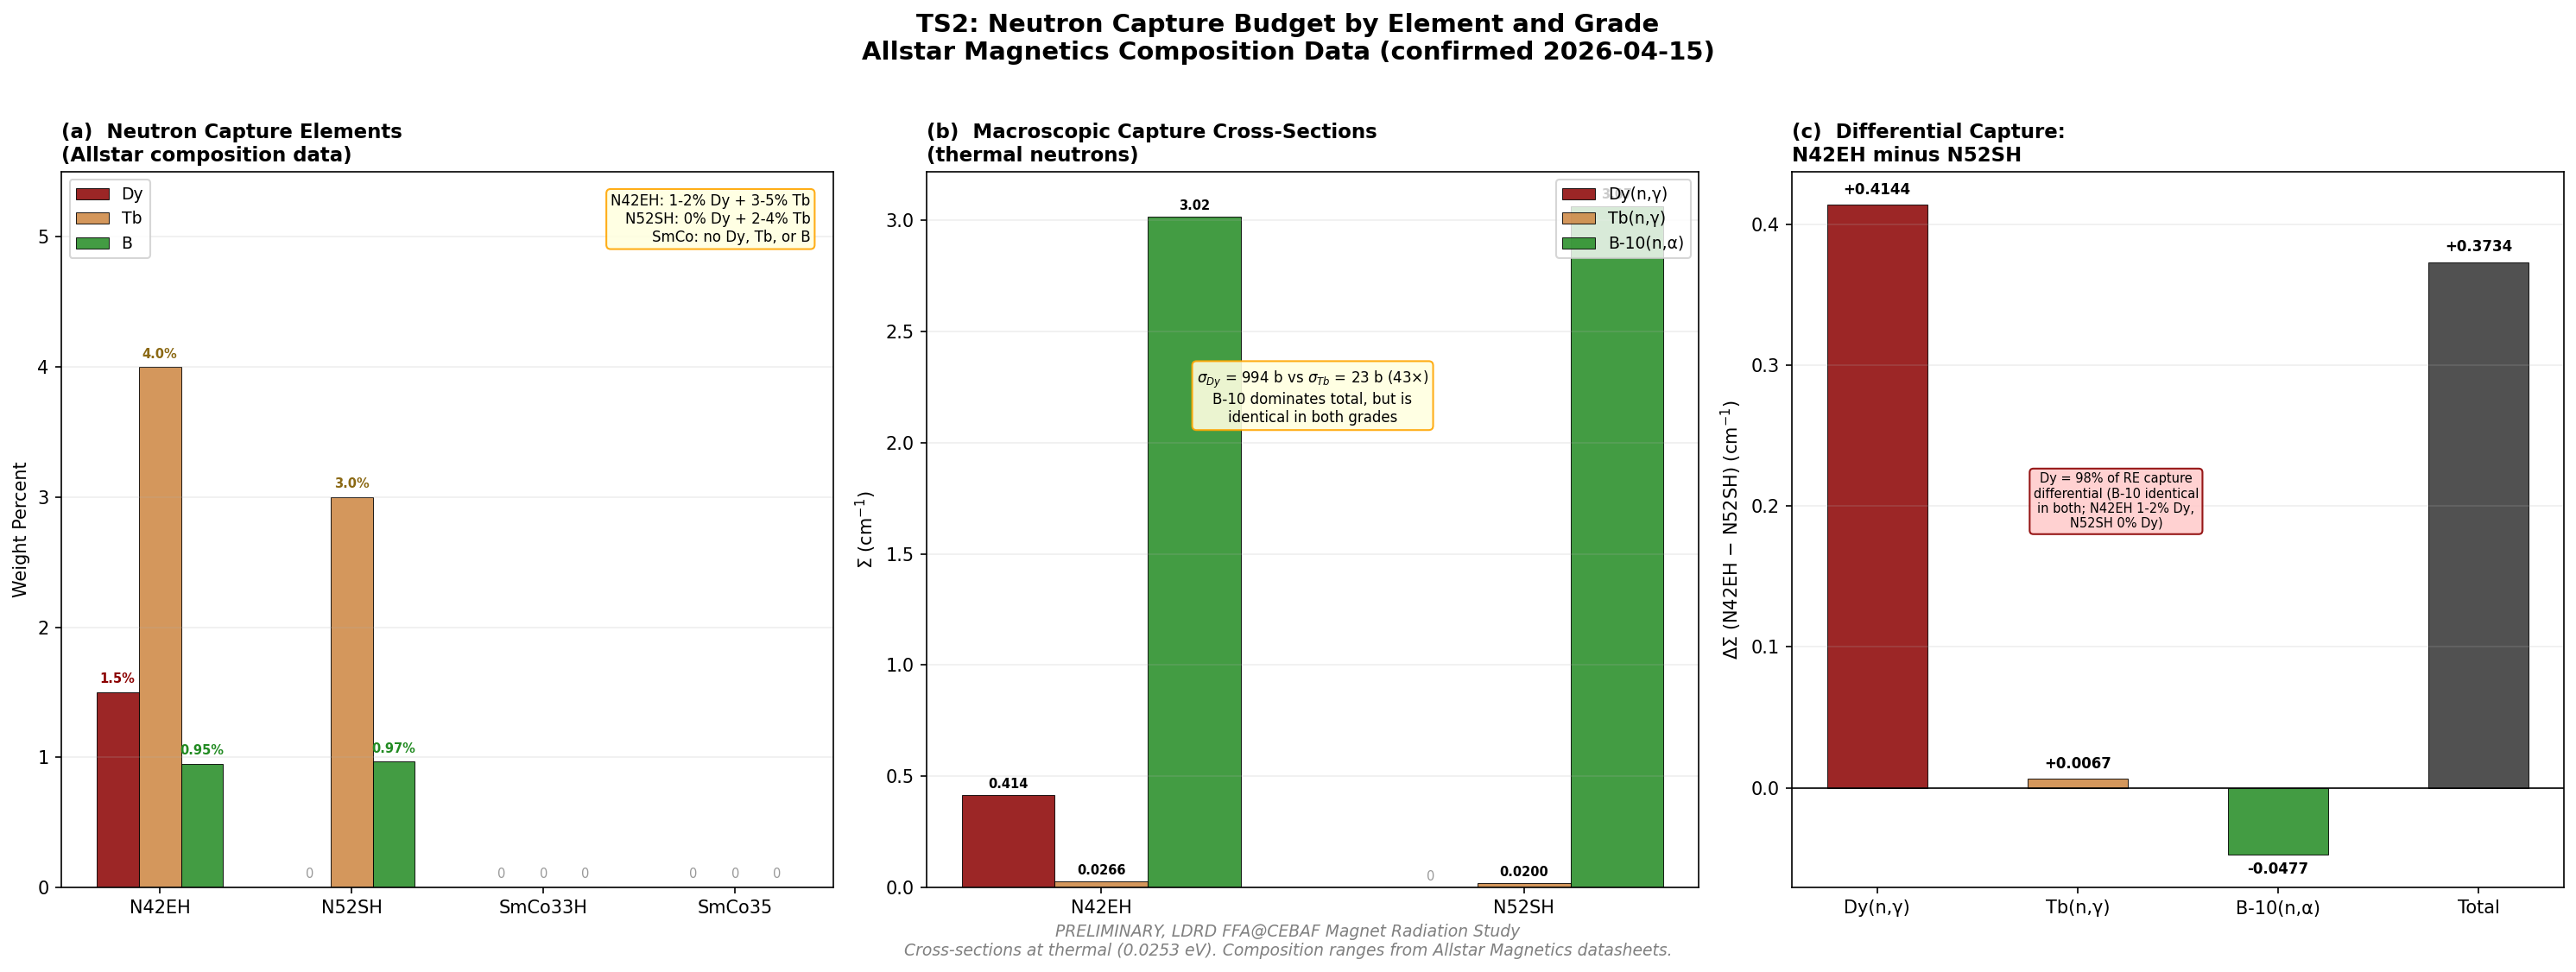
\includegraphics[width=0.95\textwidth]{figures/neutron_capture_TS2.png}
    \caption{\textbf{TS2: Neutron capture budget.}
    (a)~Weight percent of neutron-capture elements by grade (from Allstar composition data).
    (b)~Macroscopic thermal neutron capture cross-sections for the two NdFeB grades.
    (c)~Differential capture cross-section (N42EH minus N52SH), showing that Dy accounts
    for 98\% of the rare-earth capture difference, with B-10 content essentially identical.}
    \label{fig:TS2}
\end{figure}

% ============================================================================
\section{Literature Context}
\label{sec:literature}
% ============================================================================

\subsection{Prior Studies}

The radiation damage literature for permanent magnets spans several decades.
The key studies, organized by relevance to our work, are:

\begin{description}[style=nextline]
    \item[Shen et al.\ \cite{Shen2018}]
    The most-cited modern review. Catalogues demagnetization results from
    multiple facilities and concludes that neutron-induced damage (via thermal
    spikes and displacement cascades) dominates at all relevant accelerator
    dose levels, with gamma contributing primarily through secondary effects at
    very high doses.

    \item[Simos et al.\ \cite{Simos2018}]
    The closest prior NdFeB/SmCo co-irradiation study. Irradiated
    $\mathrm{Nd_2Fe_{14}B}$, $\mathrm{Pr_2Fe_{14}B}$, and
    $\mathrm{Sm_2Co_{17}}$ in spallation irradiation fields at BNL. Results:
    $\mathrm{Nd_2Fe_{14}B}$ lost $>$85\% flux at \SI{500}{kGy};
    $\mathrm{Pr_2Fe_{14}B}$ lost $>$87\% at \SI{100}{kGy}; $\mathrm{Sm_2Co_{17}}$
    showed no effect at \SI{20}{MGy}. Key difference from our work: their
    doses are 10--1000$\times$ higher, their sample size is $N = 3$, and they
    used dedicated irradiation targets rather than parasitic tunnel exposure.

    \item[Bizen et al.\ (2016) \cite{Bizen2016}]
    Landmark discovery of the magnetization reversal mechanism in NdFeB
    undulator magnets exposed to \SI{8}{GeV} electron beams. Observed $>$30\%
    flux loss at $\sim$\SI{100}{kGy} and demonstrated that damage occurs via
    localized domain reversal, not uniform demagnetization.

    \item[Bizen et al.\ (2018) \cite{Bizen2018}]
    Showed that tilting the easy axis of magnetization by \SI{45}{\degree}
    improves radiation resistance by $\sim$$10\times$, providing direct
    evidence for the thermal spike model's dependence on the relationship
    between demagnetizing field and coercive force.

    \item[Alderman et al.\ \cite{Alderman}]
    Irradiated NdFeB with pure gamma radiation (APS bending magnet
    synchrotron radiation) up to \SI{7}{MGy} and observed \textbf{no
    measurable demagnetization}. This is the highest-dose gamma-only null
    result in the literature and strongly supports our gamma-null finding.

    \item[APS LS-290 \cite{APSLS290}]
    Established that the 1\% demagnetization threshold for NdFeB varies from
    \SI{760}{Gy} to \SI{113}{kGy} depending on coercivity, geometry, and
    magnetization direction. This threshold applies under mixed (neutron-rich)
    fields; under gamma-only fields, thresholds are orders of magnitude higher.
\end{description}

\subsection{What Makes Our Study Unique}

No single prior study combines all of the following features; ours is the
first to achieve all simultaneously:

\begin{enumerate}
    \item \textbf{Co-located NdFeB/SmCo differential}: Using SmCo as an
    internal standard on the same plate enables gain-immune measurement. No
    prior study used this approach.

    \item \textbf{Sub-percent detection at $7.6\sigma$}: Prior studies either
    measure $>$1\% effects or report null results. We detect $0.208\%$ at
    high significance.

    \item \textbf{Sample size $N = 30 + 9$}: 10--$100\times$ larger than any
    prior study (typical: 2--12 samples).

    \item \textbf{Real accelerator environment}: Parasitic exposure during
    normal \CEBAF operations, not dedicated irradiation.

    \item \textbf{Low-dose regime (0.3--\SI{23451}{Gy})}: Below the threshold
    of most prior deliberate irradiation studies.

    \item \textbf{First in-situ neutron $\gg$ gamma confirmation}: The
    neutron/gamma correlation hierarchy, established by controlled experiments,
    is confirmed for the first time in a real accelerator.

    \item \textbf{Four material grades}: Statistical comparison within and
    between material families.
\end{enumerate}

\begin{figure}[H]
    \centering
    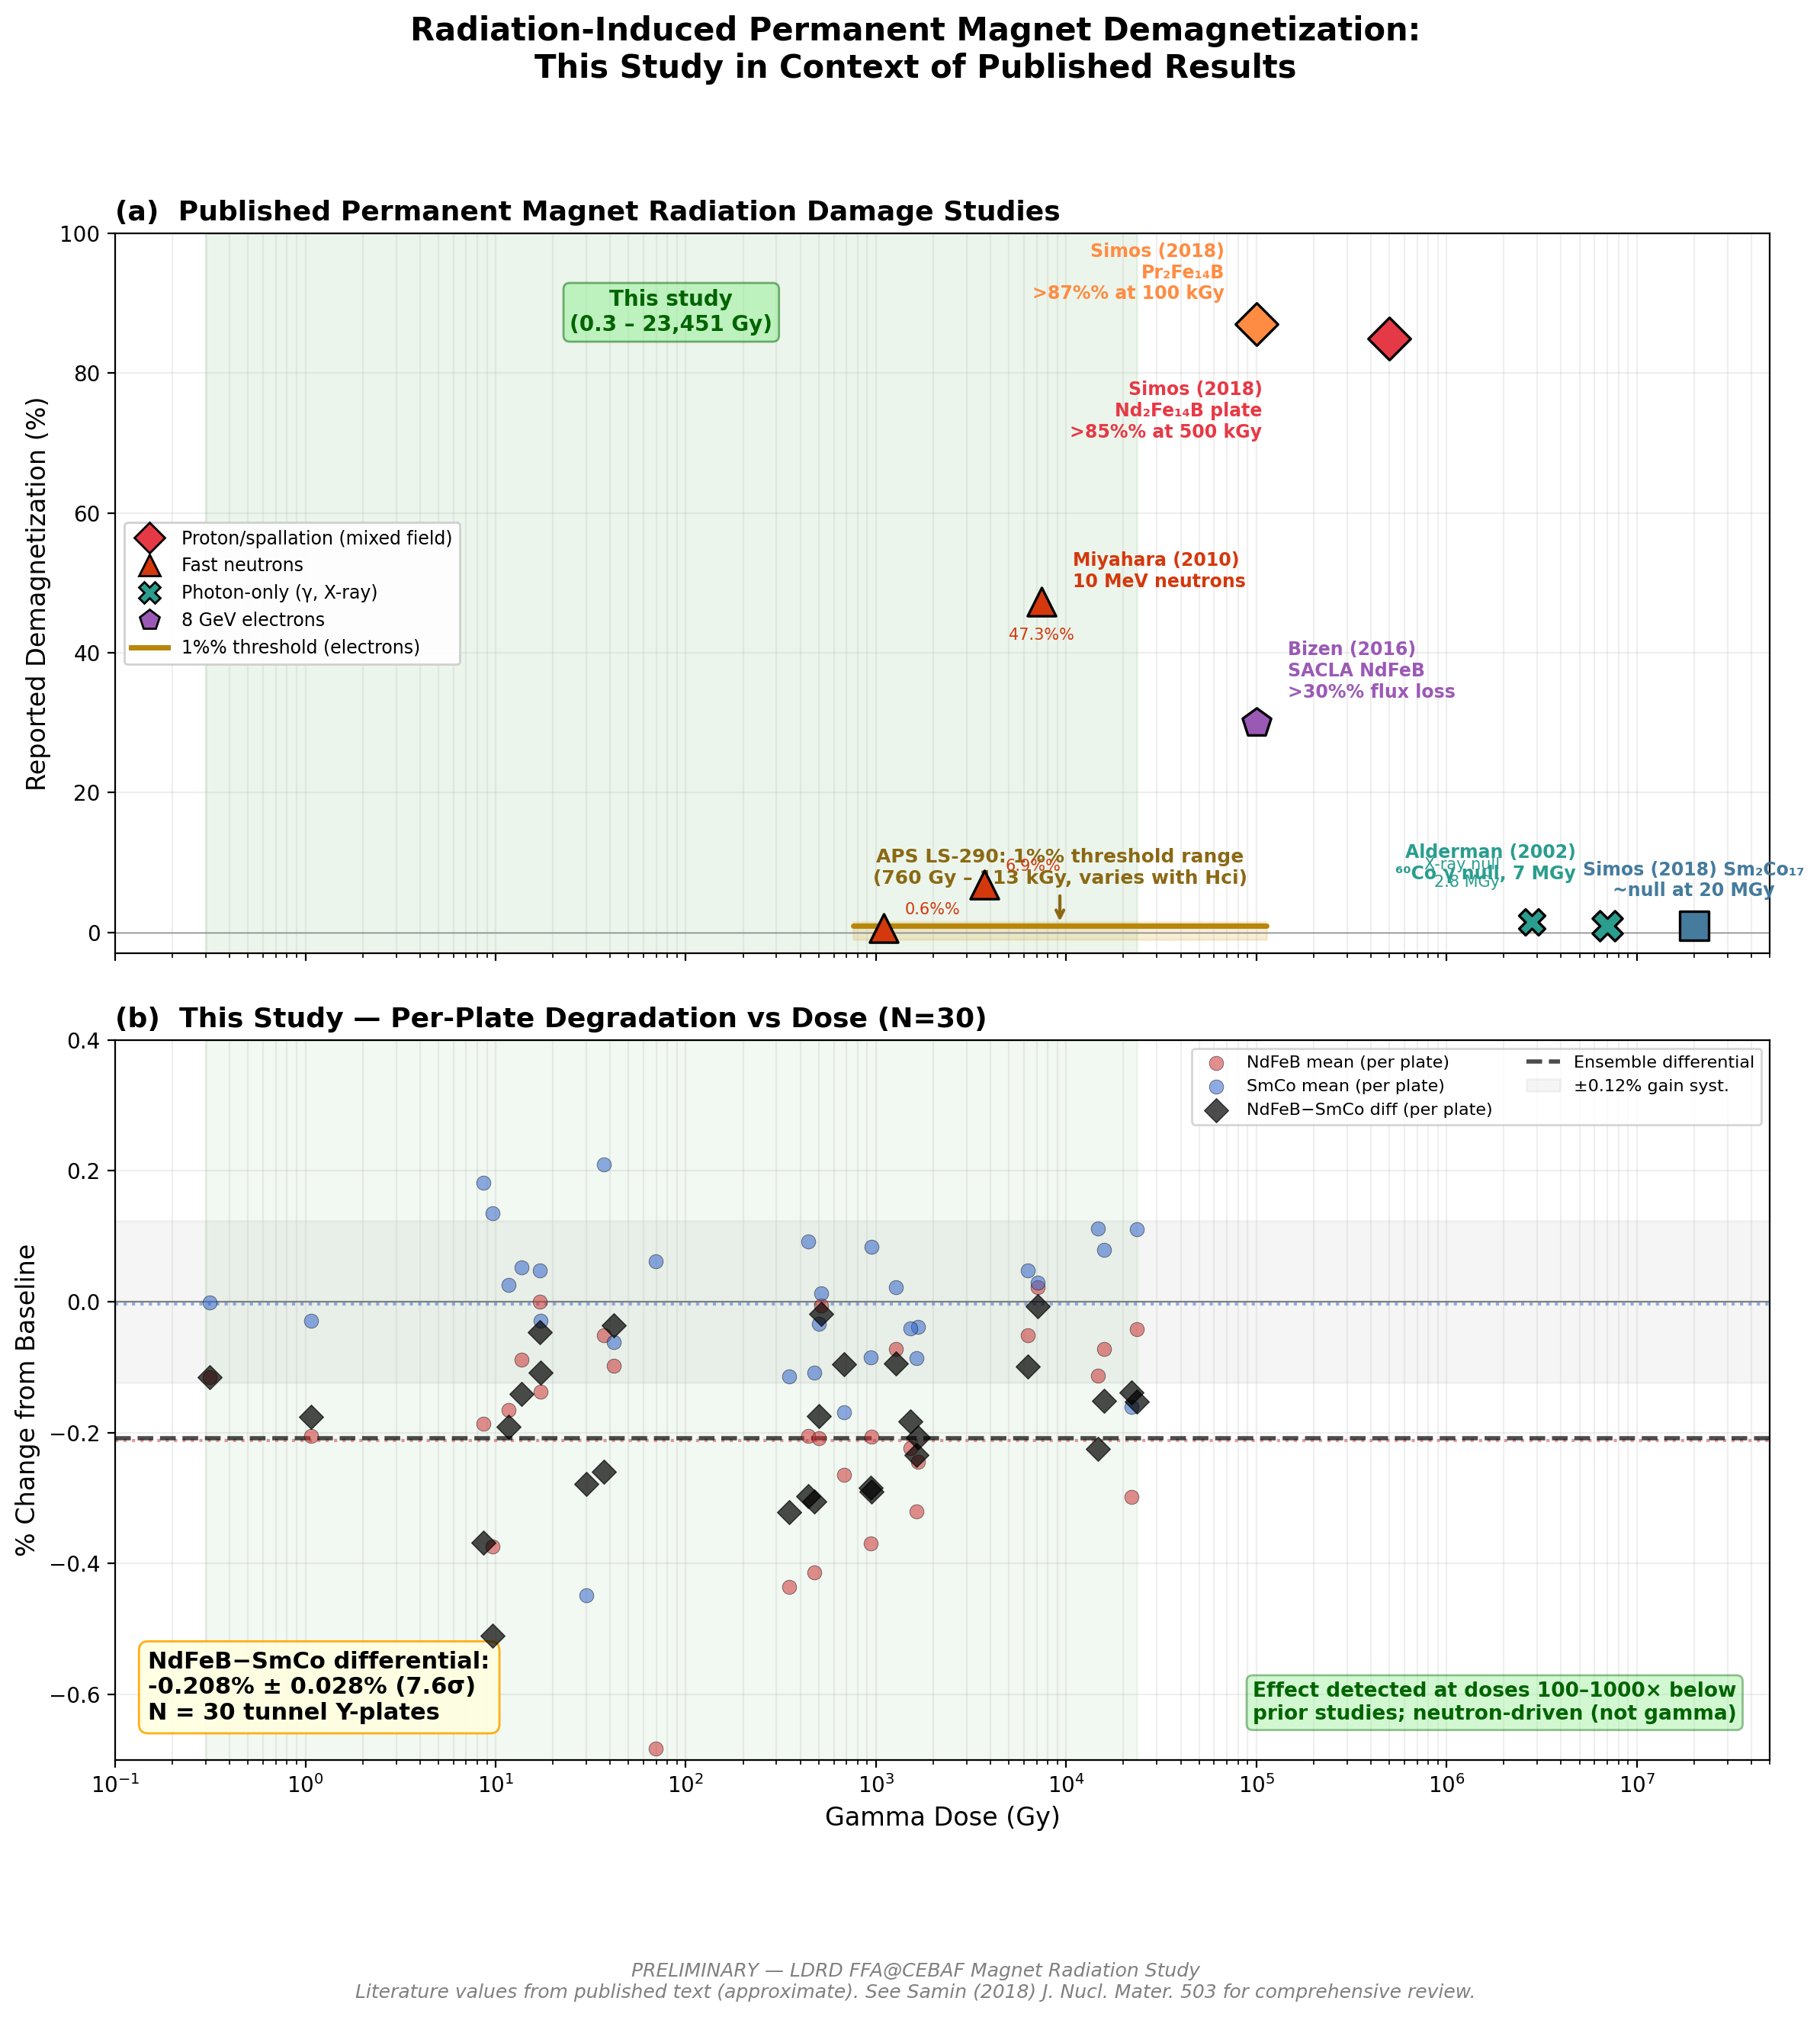
\includegraphics[width=0.95\textwidth]{figures/P15_literature_comparison.png}
    \caption{\textbf{P15: Literature comparison.} (a)~Literature landscape
    showing demagnetization from prior studies at the 0--100\% scale. Our study
    operates at doses 100--1000$\times$ below prior work. (b)~Our per-plate data
    at the sub-percent scale, showing clear NdFeB degradation and SmCo null.
    The gain-immune differential technique is what makes detection possible at
    this sensitivity.}
    \label{fig:P15}
\end{figure}

% ============================================================================
\section{Remaining Work and Future Directions}
\label{sec:future}
% ============================================================================

All tasks that can be completed with existing data have been completed. The
remaining work is blocked on external data sources or requires new
experimental campaigns.

\subsection{Blocked on External Data}

\begin{description}[style=nextline]
    \item[Task 6 (continued): Honeywell Lab Temperature Data]
    An independent room temperature record from the Honeywell building
    management system would definitively resolve the pre-deployment baseline
    temperature, which is the dominant systematic. No historical data currently exists;
    tracking must begin prospectively.

    \item[Task 12: Dysprosium Weight Percent --- RESOLVED]
    Allstar Magnetics provided composition data (April~15, 2026), confirming
    N42EH contains 1--2\,wt\%\,Dy while N52SH has zero.
    Quantitative analysis in Section~\ref{sec:n42eh_inversion}.

    \item[Task 14: NDX Neutron Dose Data]
    Complete Part\# $\to$ Area Number $\to$ location mapping for the NDX
    neutron detector data would provide a second, independent neutron dose
    measurement. Only 78/1330 badge locations are currently mapped.

    \item[Task 15: Pass-Number Trend Resolution]
    Once NDX data is available, a proper analysis of degradation vs.\ beam
    pass number would test Hypothesis~1 for the dose--position inversion.

    \item[Task 16: Beam Pass Schedule]
    The actual beam delivery schedule (which passes, how much current, for
    how long) during the exposure period would enable quantitative modeling
    of beam loss and dose at each plate position.
\end{description}

\subsection{Publication-Tier Future Tasks}

\begin{description}[style=nextline]
    \item[T2-1: NDX Neutron Dose-Response Curve (blocked on Task~14)]
    Building a proper dose-response curve (differential vs.\ neutron fluence)
    would be transformative. If monotonic, it makes the paper a candidate for
    \textit{Physical Review Letters} rather than \textit{Nuclear Instruments
    and Methods}.

    \item[T3-1: Resolve Dy-Content Hypothesis --- COMPLETE]
    Allstar composition data confirms N42EH has 1--2\,wt\%\,Dy while N52SH
    has zero. Quantitative neutron capture budget (Section~\ref{sec:n42eh_inversion},
    Figure~\ref{fig:TS2}) shows Dy accounts for 98\% of the rare-earth
    capture differential. This is a mechanistic discovery with design implications.

    \item[T3-2: Dedicated Temperature Coefficient Measurement]
    A controlled temperature sweep in the Helmholtz coil without removing
    magnets from the jig would directly measure $\alphar$ for these specific
    samples, eliminating the dominant systematic.

    \item[T3-3: Second Exposure Period]
    Returning the magnets to the tunnel for a second $\sim$18-month exposure
    would test whether the differential deepens, providing definitive proof
    of cumulative, dose-dependent damage.

    \item[T3-4: BDSIM/GEANT4 Neutron Spectrum Simulation]
    Monte Carlo simulation of the neutron fluence and energy spectrum at each
    plate location, using \CEBAF beam loss models, would:
    \begin{itemize}
        \item Predict degradation at each position from first principles
        \item Test Hypothesis~1 (beam pass structure) quantitatively
        \item Connect the measurement to the accelerator physics community
    \end{itemize}

    \item[T3-5: Resolve H-Plate Configuration Differences for Halbach Design]
    The H-plate configurations were designed as Halbach array proxies:
    Alpha ($0^\circ$, aligned), Beta ($180^\circ$, antiparallel), Gamma
    ($90^\circ$, perpendicular), and Delta (single pair with slug). If
    baseline systematics are resolved (multi-point baselines, Honeywell
    temperature data, or a second exposure campaign with improved protocols),
    comparing degradation rates across these three orientations would directly
    reveal whether field alignment relative to neighbors affects the damage
    rate. This would be one of the most important inputs for Halbach magnet
    design decisions~\cite{NGotta2024}. The A-samples within each H-plate
    provide additional per-wedge granularity for this comparison.
\end{description}

\subsection{Publication Readiness}

Based on the comprehensive peer review (April~3, 2026):

\begin{itemize}
    \item \textbf{All Tier~1 tasks are complete}: Headline consistency, error
    bar definitions, literature comparison figure, dose--position analysis,
    multiple comparisons context, temperature label, time series plots,
    fast/thermal neutron analysis.

    \item \textbf{All unblocked Tier~2 tasks are complete}: Thermal spike
    model comparison, gamma null framing, blind analysis statement, data
    dictionary update.

    \item \textbf{The paper is NIM-A or PRAB ready now.} Submission to
    \textit{Nuclear Instruments and Methods in Physics Research A} or
    \textit{Physical Review Accelerators and Beams} can proceed with the
    current analysis.

    \item \textbf{PRL requires T2-1}: A monotonic neutron dose-response curve
    would elevate the result to \textit{Physical Review Letters} significance.
\end{itemize}

% ============================================================================
\section{Summary and Conclusions}
\label{sec:conclusions}
% ============================================================================

\subsection{The Signal Is Real}

The NdFeB--SmCo differential of $-0.208\% \pm 0.028\%$~(stat) is significant
at:
\begin{itemize}
    \item \textbf{$7.6\sigma$ statistical} (from 30 intra-plate measurements)
    \item \textbf{$4.6\sigma$ combined} (including $\pm 0.033\%$ temp +
    $\pm 0.014\%$ $\alphar$ systematics in quadrature)
    \item \textbf{$4.3\sigma$ independently} from the tunnel--lab excess
    comparison
\end{itemize}

\subsection{Robust Across All Reasonable Temperatures}

The signal exceeds $5\sigma$ for any baseline temperature in the
\SIrange{23}{25}{\celsius} range. The question is magnitude, not existence.

\subsection{Lab Controls Independently Confirm}

Lab Y-plates show zero material-dependent bias ($-0.007\% \pm 0.038\%$),
proving the measurement system is clean. The $4.3\sigma$ tunnel--lab excess
uses a completely different statistical test.

\subsection{Neutron-Dominated Damage, Consistent with Theory}

\begin{itemize}
    \item Gamma dose (0.3--\SI{23451}{Gy}): no correlation ($\rho = 0.21$,
    $p = 0.27$)
    \item Neutron dose: significant correlation ($\rho = 0.389$, $p = 0.03$)
    \item Fast neutrons correlate more strongly than thermal
    \item SmCo immune, NdFeB degraded, exactly as the thermal spike model
    predicts
    \item First in-situ accelerator confirmation of the neutron $\gg$ gamma
    hierarchy
\end{itemize}

\subsection{Implications for FFA at CEBAF}

\subsubsection{What This Study Establishes}

This study establishes three findings relevant to the \FFA upgrade:
\begin{enumerate}
    \item \textbf{Radiation-induced demagnetization occurs} at \CEBAF dose
    levels. The effect is real and statistically significant. Literature
    strongly suggests it is cumulative with fluence, though confirming this
    for our samples requires a second exposure period (T3-3).
    \item \textbf{Neutrons, not gammas, correlate with the damage.} Neutron
    fluence (especially fast neutron fluence) is the critical parameter;
    gamma dose alone is not the relevant figure of merit for magnet placement
    decisions. This is consistent with the established particle hierarchy
    but is correlational in our data, not a direct causal proof.
    \item \textbf{Dysprosium content correlates with increased damage}:
    N42EH (1--2\,wt\%\,Dy) degrades more than N52SH (zero Dy), despite its
    higher intrinsic coercivity. In high-coercivity NdFeB grades, Dy is
    commonly added via the grain boundary diffusion (GBD) process,
    concentrating it at grain boundaries where neutron capture
    (43$\times$ more effective per atom than Tb) would preferentially
    disrupt the coercivity-bearing phase. If this mechanism is confirmed,
    low-Dy or Dy-free NdFeB grades would be preferred in radiation
    environments.
\end{enumerate}

These are observational findings with strong mechanistic implications.
Translating them into quantitative
predictions for \FFA magnet performance requires additional considerations
discussed below.

\subsubsection{From Bulk Remanence to Halbach Field Quality}

Our measurement is of \emph{bulk} remanence change, averaged over each
sample. For an \FFA lattice using Halbach-style combined-function magnets,
the design-relevant quantity is not the average remanence loss but rather
the resulting change in \emph{field quality} (multipole content) experienced
by the beam. Several factors make this distinction critical:

\begin{enumerate}
    \item \textbf{Non-uniform degradation within Halbach arrays.}
    Adjacent wedges in a Halbach array carry reverse flux and are not
    equivalently exposed. The side of each wedge more exposed to radiation
    and/or heat will degrade more than the shielded side, creating an
    \emph{intra-magnet gradient} that our per-sample average
    understates~\cite{NGotta2024,Brooks2017}. Even sub-percent average
    degradation can produce significant changes in the higher-order
    multipole content (sextupole, octupole, etc.) of the generated field.

    \item \textbf{Multifunction magnets are especially vulnerable.}
    \FFA magnets are inherently multifunction by design (dipole + quadrupole,
    or dipole + quadrupole + sextupole). Uneven degradation shifts the
    \emph{ratio} between these functions, not just their magnitude. If the
    dipole and quadrupole components degrade at different rates (which
    non-uniform exposure would cause), the resulting tune shifts or
    chromaticity changes could be significant even when the individual
    degradation numbers are small.

    \item \textbf{Collective effects over many cells.}
    \FFA@\CEBAF comprises more than 70 cells per ring. A single cell with a
    small field perturbation may be tolerable, but similar (though not
    identical) perturbations in every cell are magnified through the lattice.
    Systematic patterns, such as all inner-arc wedges degrading more than
    outer-arc wedges, would be particularly harmful to beam stability.
\end{enumerate}

N'Gotta et al.~\cite{NGotta2024} have studied Halbach degradation patterns
and their lattice-level impacts, and are developing physically adjustable
wedge inserts (``magic fingers'') within Halbach arrays to tune optics and
compensate for radiation-induced field quality changes. Brooks~\cite{Brooks2017}
has shown non-uniform demagnetization patterns within Halbach arrays and
their implications for multipole field quality in FFA lattices. Dedicated
simulation (mapping a degradation profile onto each wedge, computing
multipole errors, and tracking through the lattice) is needed to determine
whether the degradation levels measured in this study are tolerable for the
\FFA design.

\subsubsection{Material Selection Considerations}

\textbf{SmCo:} While SmCo shows zero measurable degradation and is the
radiation-hardest candidate, it carries significant operational drawbacks
that must be weighed against its radiation resistance:
\begin{itemize}
    \item \textbf{Brittleness}: \SmCo{} is extremely brittle, creating
    fracture risk during handling, installation, and maintenance of large
    magnet arrays.
    \item \textbf{Lower remanence}: SmCo achieves $\Br \approx$
    11.2--\SI{12.0}{kGs} compared to 12.8--\SI{14.5}{kGs} for NdFeB,
    requiring larger or more magnets for equivalent integrated field.
    \item \textbf{Neutron activation}: Samarium and cobalt have significant
    neutron activation cross-sections. In a high-fluence environment, SmCo
    magnets may become activated over time, potentially requiring handling
    protocols that add to maintenance complexity and personnel dose.
\end{itemize}
SmCo may therefore not be a viable candidate for all \FFA applications
despite its radiation hardness, and operational safety considerations
may ultimately constrain the material choice.

\textbf{NdFeB:} If NdFeB is used, the data suggest: prefer low-Dy or
Dy-free grades (e.g., N52SH over N42EH), use neutron fluence rather than
gamma dose as the relevant siting parameter, and plan for periodic
monitoring of field quality.

\subsubsection{The H-Sample Configurations as a Path Forward}

The H-plate configurations (Alpha, Beta, Gamma, Delta) were designed as
Halbach array proxies: Alpha ($0^\circ$, aligned) represents parallel-flux
regions, Beta ($180^\circ$, antiparallel) simulates adjacent reverse-flux
wedges, and Gamma ($90^\circ$, perpendicular) probes the intermediate
orientation. Delta (single pair with slug) serves as a baseline reference.
If baseline systematics can be resolved (Section~\ref{sec:future}),
comparing degradation rates across these three orientations would directly
reveal whether field alignment affects the damage rate, providing critical
input for Halbach design. This is one of the most important goals for
future analysis (Section~\ref{sec:future}).

% ============================================================================
\section*{Acknowledgments}
% ============================================================================

[Placeholder for acknowledgments: Allstar Magnetics, JLab RADCON, Kirsten
(dosimetry), JLab Operations, LDRD program.]

% ============================================================================
% APPENDICES
% ============================================================================
\newpage
\begin{appendices}

\section{Complete Plot Inventory}
\label{app:plots}

The following figures were generated as part of this study. All are included
in the \texttt{Technical\_Note/figures/} directory.

\subsection{Presentation Plots (P1--P15)}
\begin{description}
    \item[P1] Material comparison (4 grades, tunnel Y-plates)
    \item[P2] Time series by material (3 panels: NdFeB, SmCo, differential)
    \item[P3] Regional breakdown (by tunnel region)
    \item[P4] Lab control comparison
    \item[P5] Uncertainty budget table
    \item[P6] $\Delta T_\mathrm{crit}$ vs.\ observed degradation
    \item[P7] Teslameter summary
    \item[P8] Waterfall by region
    \item[P9] Waterfall all materials
    \item[P10] H-plate material comparison
    \item[P11] A-sample summary
    \item[P12] Combined Y/H/A comparison
    \item[P13] H/A lab vs.\ tunnel
    \item[P14] Co-located cross-reference
    \item[P15] Literature comparison (2 panels)
\end{description}

\subsection{Rod Dosimetry Plots (R1--R7, C1, TS1)}
\begin{description}
    \item[R1] Gamma/neutron dose vs.\ NdFeB degradation (side-by-side)
    \item[R2] Dose--degradation by material grade
    \item[R3] Differential vs.\ dose (gamma and neutron)
    \item[R4] Regional dose--degradation patterns
    \item[R5] Dose comparison (OSL vs.\ AIdata)
    \item[R6] Fast vs.\ thermal neutron correlations ($2\times 3$ grid)
    \item[R7] Dose--position inversion (3 panels)
    \item[C1] FWT-70 calibration curves (4 OD-to-dose fits)
    \item[TS1] Thermal spike model comparison (3 panels)
    \item[TS2] Neutron capture budget by element and grade (3 panels)
\end{description}

\subsection{Time Series Plots (T1--T7)}
\begin{description}
    \item[T1] Ensemble mean vs.\ time (2 panels: full + zoomed)
    \item[T2] Spaghetti trajectories (all individual plates)
    \item[T3] Degradation vs.\ dose, time-resolved
    \item[T4] Regional time evolution
    \item[T5] Dose accumulation by region
    \item[T6] Degradation and dose by region (joint panel)
    \item[T7] Per-plate dose timeline
\end{description}

\subsection{Other Plots}
\begin{description}
    \item[U1] Grand comparison (tunnel vs.\ lab, all sample types)
    \item[U2] Strip plot (all types)
    \item[U3] Forest plot (effect sizes)
    \item[S1] Temperature sensitivity sweep
    \item[S2] Sample type comparison (Y vs.\ H vs.\ A)
    \item[S3] Trajectory comparison
\end{description}

\section{Glossary of Key Terms}
\label{app:glossary}

\begin{description}
    \item[A-sample] Individual magnet pair extracted from an H-plate assembly.
    Named An-XX-Y-Z or As-XX-Y-Z.
    \item[$\alphar$] Temperature coefficient of remanence (\%/\si{\celsius}).
    Describes how the magnetic moment changes with temperature.
    \item[AIdata] Kirsten's pre-integrated cumulative dose database, derived
    from FWT-70 optichromic rod readings.
    \item[$\Br$] Remanence. The residual magnetic flux density when the
    external field is removed.
    \item[CR-39] Columbia Resin \#39. A nuclear track-etch detector used for
    neutron dosimetry. Fast neutrons create recoil proton tracks; thermal
    neutrons interact via converter foils.
    \item[Curie temperature ($\Tc$)] Temperature above which a ferromagnet
    loses its spontaneous magnetization. $\sim$\SI{588}{K} for NdFeB,
    $\sim$\SI{1093}{K} for SmCo.
    \item[FFA] Fixed Field Alternating-gradient. An accelerator optics concept
    using permanent magnets with gradient fields to transport beams of
    multiple energies.
    \item[FWT-70] Far West Technology Model~70. An optichromic (color-change)
    film dosimeter for gamma radiation, read spectrophotometrically.
    \item[Gain drift] Session-to-session variation in the Helmholtz coil
    fluxmeter's sensitivity, typically 0.5--0.7\%.
    \item[$\Ha$] Anisotropy field. The internal magnetic field associated with
    crystalline anisotropy. Higher $\Ha$ means harder domain reversal.
    \item[$\Hci$] Intrinsic coercivity. The reverse field needed to
    demagnetize the material. Higher $\Hci$ generally means more radiation
    resistance (with caveats).
    \item[Helmholtz coil] A pair of identical coils producing a uniform field
    region, used with a fluxmeter to measure magnetic moment.
    \item[H-plate] Pair assembly containing magnets in a specific magnetic
    configuration: Alpha ($0^\circ$), Beta ($180^\circ$), Gamma ($90^\circ$),
    or Delta (single pair + slug). Measured with Helmholtz coil.
    \item[Intra-plate differential] The NdFeB mean minus SmCo mean computed
    within a single Y-plate. Gain-immune by construction.
    \item[mWC] milliWeber-centimeter. Unit of the Helmholtz coil flux integral,
    proportional to magnetic moment.
    \item[NDX] Neutron detector. Facility instrument at specific tunnel
    locations that measures beam loss rates.
    \item[OSL] Optically Stimulated Luminescence. Dosimetry technique using
    stored charge in crystalline materials. Saturates at \SI{1000}{rad}.
    \item[PKA] Primary Knock-on Atom. The first atom displaced by an incident
    neutron, initiating a displacement cascade.
    \item[SEM] Standard Error of the Mean. $\mathrm{SEM} = \sigma / \sqrt{N}$.
    All error bars in this study represent $\pm 1$~SEM unless noted.
    \item[Spearman $\rho$] Non-parametric rank correlation coefficient.
    Measures monotonic (not necessarily linear) association between two
    variables.
    \item[Thermal spike] A nanoscale region locally heated above $\Tc$ by a
    displacement cascade, causing irreversible domain reversal.
    \item[Y-plate] Large single magnet with 4 material slots (one each of
    N42EH, N52SH, SmCo33H, SmCo35). Primary measurement unit.
\end{description}

\section{Data File Inventory}
\label{app:data_files}

The complete data package (\texttt{Data\_Package/}) contains:

\begin{longtable}{@{}p{6cm}p{8cm}@{}}
\toprule
\textbf{File} & \textbf{Description} \\
\midrule
\endhead
\multicolumn{2}{l}{\textit{01\_Sample\_Configuration/}} \\
\quad materials\_arrangements.csv & Material assignment for every magnet slot \\
\quad tunnel\_placements.csv & Physical location of each tunnel plate \\
\quad sample\_inventory.csv & Complete sample list \\
\midrule
\multicolumn{2}{l}{\textit{02\_Magnetic\_Measurements/}} \\
\quad y\_plate\_degradation.csv & Primary Y-plate results (30+9 plates) \\
\quad h\_plate\_degradation.csv & H-plate pair results \\
\quad a\_sample\_degradation.csv & A-sample individual results \\
\quad y\_plate\_time\_series.csv & Per-date percentage changes \\
\quad temperature\_corrections.csv & Temperature correction details \\
\midrule
\multicolumn{2}{l}{\textit{03\_Dosimetry/}} \\
\quad plate\_cumulative\_dose.csv & AIdata rod doses per plate \\
\quad merged\_dose\_final.csv & Authoritative merged doses \\
\quad master\_doses.csv & Full OSL badge database \\
\quad rod\_doses.csv & Optichromic rod measurements \\
\quad neutron\_breakdown.csv & Thermal/fast neutron split \\
\quad dose\_vs\_degradation.csv & Merged dose + degradation \\
\quad rod\_dose\_degradation.csv & Extended merge with uncertainties \\
\quad rod\_uncertainty\_budget.csv & Per-plate uncertainty budget \\
\midrule
\multicolumn{2}{l}{\textit{04\_Results/}} \\
\quad headline\_results.csv & Key results in machine-readable format \\
\midrule
\multicolumn{2}{l}{\textit{05\_Plots/}} \\
\quad & 40+ plots in presentation/, time\_series/, rod\_dosimetry/, other/ \\
\midrule
\multicolumn{2}{l}{\textit{06\_Scripts/}} \\
\quad & 20+ Python scripts (reference copies) \\
\bottomrule
\end{longtable}

\end{appendices}

\printbibliography

\end{document}
